%%%%%%%%%%%%%%%%%%%%%%%%%%  ltexpprt.tex  %%%%%%%%%%%%%%%%%%%%%%%%%%%%%%%%
%
% This is ltexpprt.tex, an example file for use with the SIAM LaTeX2E
% Preprint Series macros. It is designed to provide double-column output.
% Please take the time to read the following comments, as they document
% how to use these macros. This file can be composed and printed out for
% use as sample output.

% Any comments or questions regarding these macros should be directed to:
%
%                 Donna Witzleben
%                 SIAM
%                 3600 University City Science Center
%                 Philadelphia, PA 19104-2688
%                 USA
%                 Telephone: (215) 382-9800
%                 Fax: (215) 386-7999
%                 e-mail: witzleben@siam.org


% This file is to be used as an example for style only. It should not be read
% for content.

%%%%%%%%%%%%%%% PLEASE NOTE THE FOLLOWING STYLE RESTRICTIONS %%%%%%%%%%%%%%%

%%  1. There are no new tags.  Existing LaTeX tags have been formatted to match
%%     the Preprint series style.
%%
%%  2. You must use \cite in the text to mark your reference citations and
%%     \bibitem in the listing of references at the end of your chapter. See
%%     the examples in the following file. If you are using BibTeX, please
%%     supply the bst file with the manuscript file.
%%
%%  3. This macro is set up for two levels of headings (\section and
%%     \subsection). The macro will automatically number the headings for you.
%%
%%  5. No running heads are to be used for this volume.
%%
%%  6. Theorems, Lemmas, Definitions, etc. are to be double numbered,
%%     indicating the section and the occurence of that element
%%     within that section. (For example, the first theorem in the second
%%     section would be numbered 2.1. The macro will
%%     automatically do the numbering for you.
%%
%%  7. Figures, equations, and tables must be single-numbered.
%%     Use existing LaTeX tags for these elements.
%%     Numbering will be done automatically.
%%
%%
%%%%%%%%%%%%%%%%%%%%%%%%%%%%%%%%%%%%%%%%%%%%%%%%%%%%%%%%%%%%%%%%%%%%%%%%%%%%%%%



\documentclass[twoside,leqno,twocolumn]{article}
\usepackage{ltexpprt}
\usepackage{graphicx}
\usepackage{epstopdf}
\usepackage{amsmath}
\usepackage{amssymb}
\usepackage{color}
\usepackage{epsfig}
\usepackage{tabularx}
%\usepackage{ctable}
\usepackage{multirow}
\usepackage{subfigure}
\usepackage{mathrsfs}
\usepackage{mathtools}
\usepackage{hyperref}
\usepackage{booktabs}
\usepackage{sci}
\usepackage{epstopdf}

\newenvironment{remark}{\emph{Remark.}}

\newcommand{\Songfan}[1]{\textcolor{red}{#1}}
\newcommand{\SFAdd}[1]{\textcolor{blue}{#1}}

\begin{document}


%\setcounter{chapter}{2} % If you are doing your chapter as chapter one,
%\setcounter{section}{3} % comment these two lines out.

\title{\Large Facial Expression Based Online User Behavior Analysis for Advertising Evaluation\thanks{Supported by }}
\author{Songfan Yang\thanks{Sichuan University, China} \\
\and
Le An\thanks{University of North Carolina at Chapel Hill}}
\date{}

\maketitle


%\pagenumbering{arabic}
%\setcounter{page}{1}%Leave this line commented out.

\begin{abstract} \small\baselineskip=9pt The surge of multimedia contents being made available online has attracted more and more users. As a new platform, more advertisements have been presented online due to the increased user population and reduced advertising cost. In addition, a large portion of revenue for major IT companies such as Google and Facebook is generated by online advertisements. Hence, for both advertiser and advertisement hosts, effective advertisement targeting and delivering is of great interest and importance. In this paper, we quantify users' advertisement viewing experience based on their facial expression responses and propose a metric termed moment-to-moment zapping probability (MMZP) for predicting users' ``zapping'', i.e., ``skipping'' behavior. Insights are discovered by analyzing MMZP and such knowledge may help improve the advertising effectiveness,e.g., presenting the most suitable advertisements to the user with specific attributes such as gender and ethnicity.\end{abstract}

\section{Introduction}
With the proliferation of online multimedia contents as well as the rapid growth of Internet users, broadcasting and advertising business are shifting their attention from traditional media such as TV to the Internet. As an example, the revenue from Internet advertising is expected to boost over $60\%$ to nearly $200$ billion USD from 2013 to 2018. Due to the increased audience population and reduced cost of online advertising, advertisers are more inclined to publish advertisements (ads) online. On the other hand, most popular Internet sites (e.g., Google, Facebook) depend on advertising as their major revenue source. As a result, effective advertising are important to both advertisers and advertisement hosts.

To evaluate the quality of advertising, user behavior is usually studied. Such analysis can be conducted using users' self-reported feedback. However, this approach suffers from cognitive bias and cannot provide users' dynamic feedback to the ad provider~\cite{Poels06}. Another way of evaluating ad quality is to study users' \textit{zapping} behavior. Zapping is an important metric which is defined as the action that a user stops watching an ad. Zapping implies diminished attention of the user who would less likely become a potential consumer~\cite{Elpers03}. In traditional media such as TV, zapping occurs when the user switches channel. For online advertising, the user normally has the option to zap (i.e., skip) an ad. Thus, accurately predicting and preventing zapping can lead to more effective advertising campaign. 

As suggested in~\cite{Abbasi_15}, user behavior is affected by perceptual considerations such as personal feelings; extracting such information is a challenging task. In this paper we analyze the user behavior during ad watching using their facial expression responses. As a rich source of implicit communication, facial expression reflects one's spontaneous feeling and can be measured non-intrusively~\cite{Ekman93}. \Songfan{Automatic
facial expression recognition finds its applications in human
behavior analysis, human-human interaction and human-computer
interaction. Automatic facial expressions analysis is non-intrusive and can
be dynamically analyzed as a commercial is
playing~\cite{Teixeira12}. Accurate facial expression analysis
facilitates the marketing and advertising researchers in
understanding a user's emotional state and behavior. This has
the potential to improve the effectiveness of advertising or even
design interactive commercials to enhance the advertising
experience.} Previous studies show that facial expression is correlated with zapping behavior~\cite{Yang_TAC14, Yang_FG15}.  

In this paper, to study the users' behavior in online advertising, our \textit{first} objective is to predict the moment-to-moment zapping probability (MMZP) from users' facial expression during ad watching. The MMZP reflects users' dynamic interest level to the ad content. By collecting MMZP from diverse groups of users watching ads in multiple categories, our \textit{second} objective is to extract user preference information from MMZP. To achieve these goals, we first describe a data collection paradigm and justify why ``smile'' is the expression of the central focus in analyzing users' feedback to an ad. Subsequently, we divide the smile responses into segments, which we term \textit{responselet}, and learn a dictionary of responselet. Predictions of MMZP are made by classifying the smile responses using their sparse reconstruction coefficients as features. From the predictions of MMZP, rich knowledge about user preference is discovered, which is valuable for better understanding and promoting online ads. 


\section{Related Work}

\subsection{Automatic Facial Expression Recognition.}

\Songfan{Facial expression recognition techniques can be broadly divided as geometric-based approaches, appearance-based approaches, and the combination of both.}

\Songfan{Geometric-based approaches track the facial geometry over time and infer expression based on the facial geometry deformation. Some exemplar methods include: Active Shape Model (ASM)~\cite{Hu04}, Active Appearance Model (AAM)~\cite{Lucey06}, particle filter~\cite{Valstar05}, geometric deformation~\cite{Kotsia07}. Appearance-based approaches, on the other hand, emphasize on describing the appearance of facial features and their dynamics. Whitehill et al.~\cite{Whitehill09} use a bank of Gabor energy filters to decompose the facial texture. The volume of local binary patterns (VLBP) is extracted in~\cite{Zhao07}. Yang et al.~\cite{Yang12} aggregate the dynamics of the facial expression into a single image, Emotion Avatar Image (EAI), for high accuracy person-independent expression recognition.}

\subsection{Expression Analysis for Advertising Research.}

To study the spontaneous consumer facial expressions during ad watching, an interesting study was conducted by McDuff \textit{et al.}~\cite{McDuff13} who collected naturalistic facial response from people watching the US presidential debate in 2012. They found out that voter preference can be predicted with an average accuracy of over 73\% based on facial expression responses. The AMFED dataset was introduced in~\cite{amfed}, providing both spontaneous facial expression videos and self-report responses. Although this dataset does not concern users' zapping behavior, it provides a large testbed for ``in-the-wild'' consumer ad watching expression analysis. In a more realistic case, consumers may not be cooperative and can switch away from the viewing content at any moment. Thus, it is important and challenging for advertisers to retain users' attention during the playing of an ad. \Songfan{Elpers et al.~\cite{Elpers03} demonstrate that both the entertainment and the information value of a commercial have a strong multiplicative effect on the probability for a commercial to be watched by viewers.} Teixeira \textit{et al.}~\cite{Teixeira12} analyzed the user's zapping behavior using joy and surprise expressions. They found that the joy response highly correlates with user's zapping behavior. It was suggested that retaining a user's attention can produce desirable communication effects increase his/her interest as a potential consumer. 


\section{Experimental Design}

\subsection{Facial Expression Data.}

A facial expression dataset for online advertising analysis~\cite{Yang_FG15} is used in our experiments. In this dataset, 51 subjects were invited to watch multiple ads, each of which ranges from 30 to 90 seconds. Among those subjects, 16 are female and 35 are male. Regarding ethnicity, there are 9 Caucasians, 14 Asian Americans, 18 Asians, 8 Hispanics, and 2 African Americans. When watching an ad, a user can choose to finish watching or zap before it ends. In either case, 30 seconds were allowed for the user to neutralize their emotions. The selected 8 ads in our experiments cover two most popular categories: \textit{Car} and \textit{Fast Food}. \Songfan{These two categories have less gender bias compared with categories such \textit{Beer} or \textit{Makeup}. The selected ads are from recognizable brands that have various entertaining levels based on their contents.} Here, we use a scalar from 0 to 10 to rate the entertaining level of an ad from low to high. The scores for the ads were rated by an independent group of subjects and the averaged scores are used. Table~\ref{table:ads} lists the ads information. In general the \textit{Car} ads are more entertaining than the \textit{Fast Food} ads with \textit{Toyota} and \textit{Nissan} being the two most amusing ones. All ads are available on primary websites such as YouTube. The playback order for these ads were randomized for each subject to diminish the ordering impact. 


\begin{table*}[!t]
\caption{Advertisements used in our experiments} \label{table:ads}
\centering
\scriptsize
\begin{tabular}{lllll}
\toprule
Category & Brand & Ad Name & Entertaining Level & Length (in \textit{s}) \\ \midrule

\multirow{4}{*}{Car}        & Toyota & I Wish  & 8 & 60			\\ %\cline{2-3}
                            & Honda  & We Know You  & 3 & 90 \\ %\cline{2-3}
                            & Chevy  & Wind Test  & 4 & 30  \\ %\cline{2-3}
                            & Nissan & Enough   & 9 & 30    \\ %\cmidrule{2-3}
\midrule 
\multirow{4}{*}{Fast Food} & Jack In The Box & Hot Mess               & 5 &  30 \\ %\cline{2-3}
                            & Subway                & New Footlong    & 4 & 30 \\ %\cline{2-3}
                            & Carl's Jr.            & Oreo Ice Cream  & 6 &  32 \\ %\cline{2-3}
                            & Pizza Hut             & Make It Great   & 3 & 30 \\ %\cmidrule{2-3}
\bottomrule
\end{tabular}
\end{table*} 

\subsection{Motivation for Using Smile Response.}
Among common facial expressions, such as \textit{fear} or \textit{sadness}, smile response is leveraged in our method to predict zapping behavior due to the following motivations:
\begin{itemize}
\item It is shown by Elper \textit{et al.}~\cite{Elpers03} that the lack of \textit{entertaining} factor in ads is a major reason for zapping. For the ad selection in this dataset, we focus on entertaining factor only. In addition, a large number of ads aim at amusing, so ads with various entertaining levels are widely available. 

\item In terms of facial expression response to ad watching, smile directly reflects the entertaining level of ads. It is observed that more than 95\% of the detected expressions are smile in our dataset. A similar observation is also made recently~\cite{amfed}. 

\item As an extensively studied facial expression, smile and its intensity can be accurately detected on a per frame basis and with simple features and a Support Vector Machine (SVM) classifier, smile classification can achieve an area under the curve (AUC) of 0.95~\cite{Yang_TAC14}. Examples of smile responses associated with zapping and non-zapping behavior are shown in Fig.~\ref{fig:smile_ex}. 


\end{itemize}

\begin{figure}[t] 
\centering
 \subfigure[Zapping]{\includegraphics[width=.65\columnwidth]{fig/response_seq_zap_ex}\label{fig:ex_zap}}
\subfigure[Non-zapping]{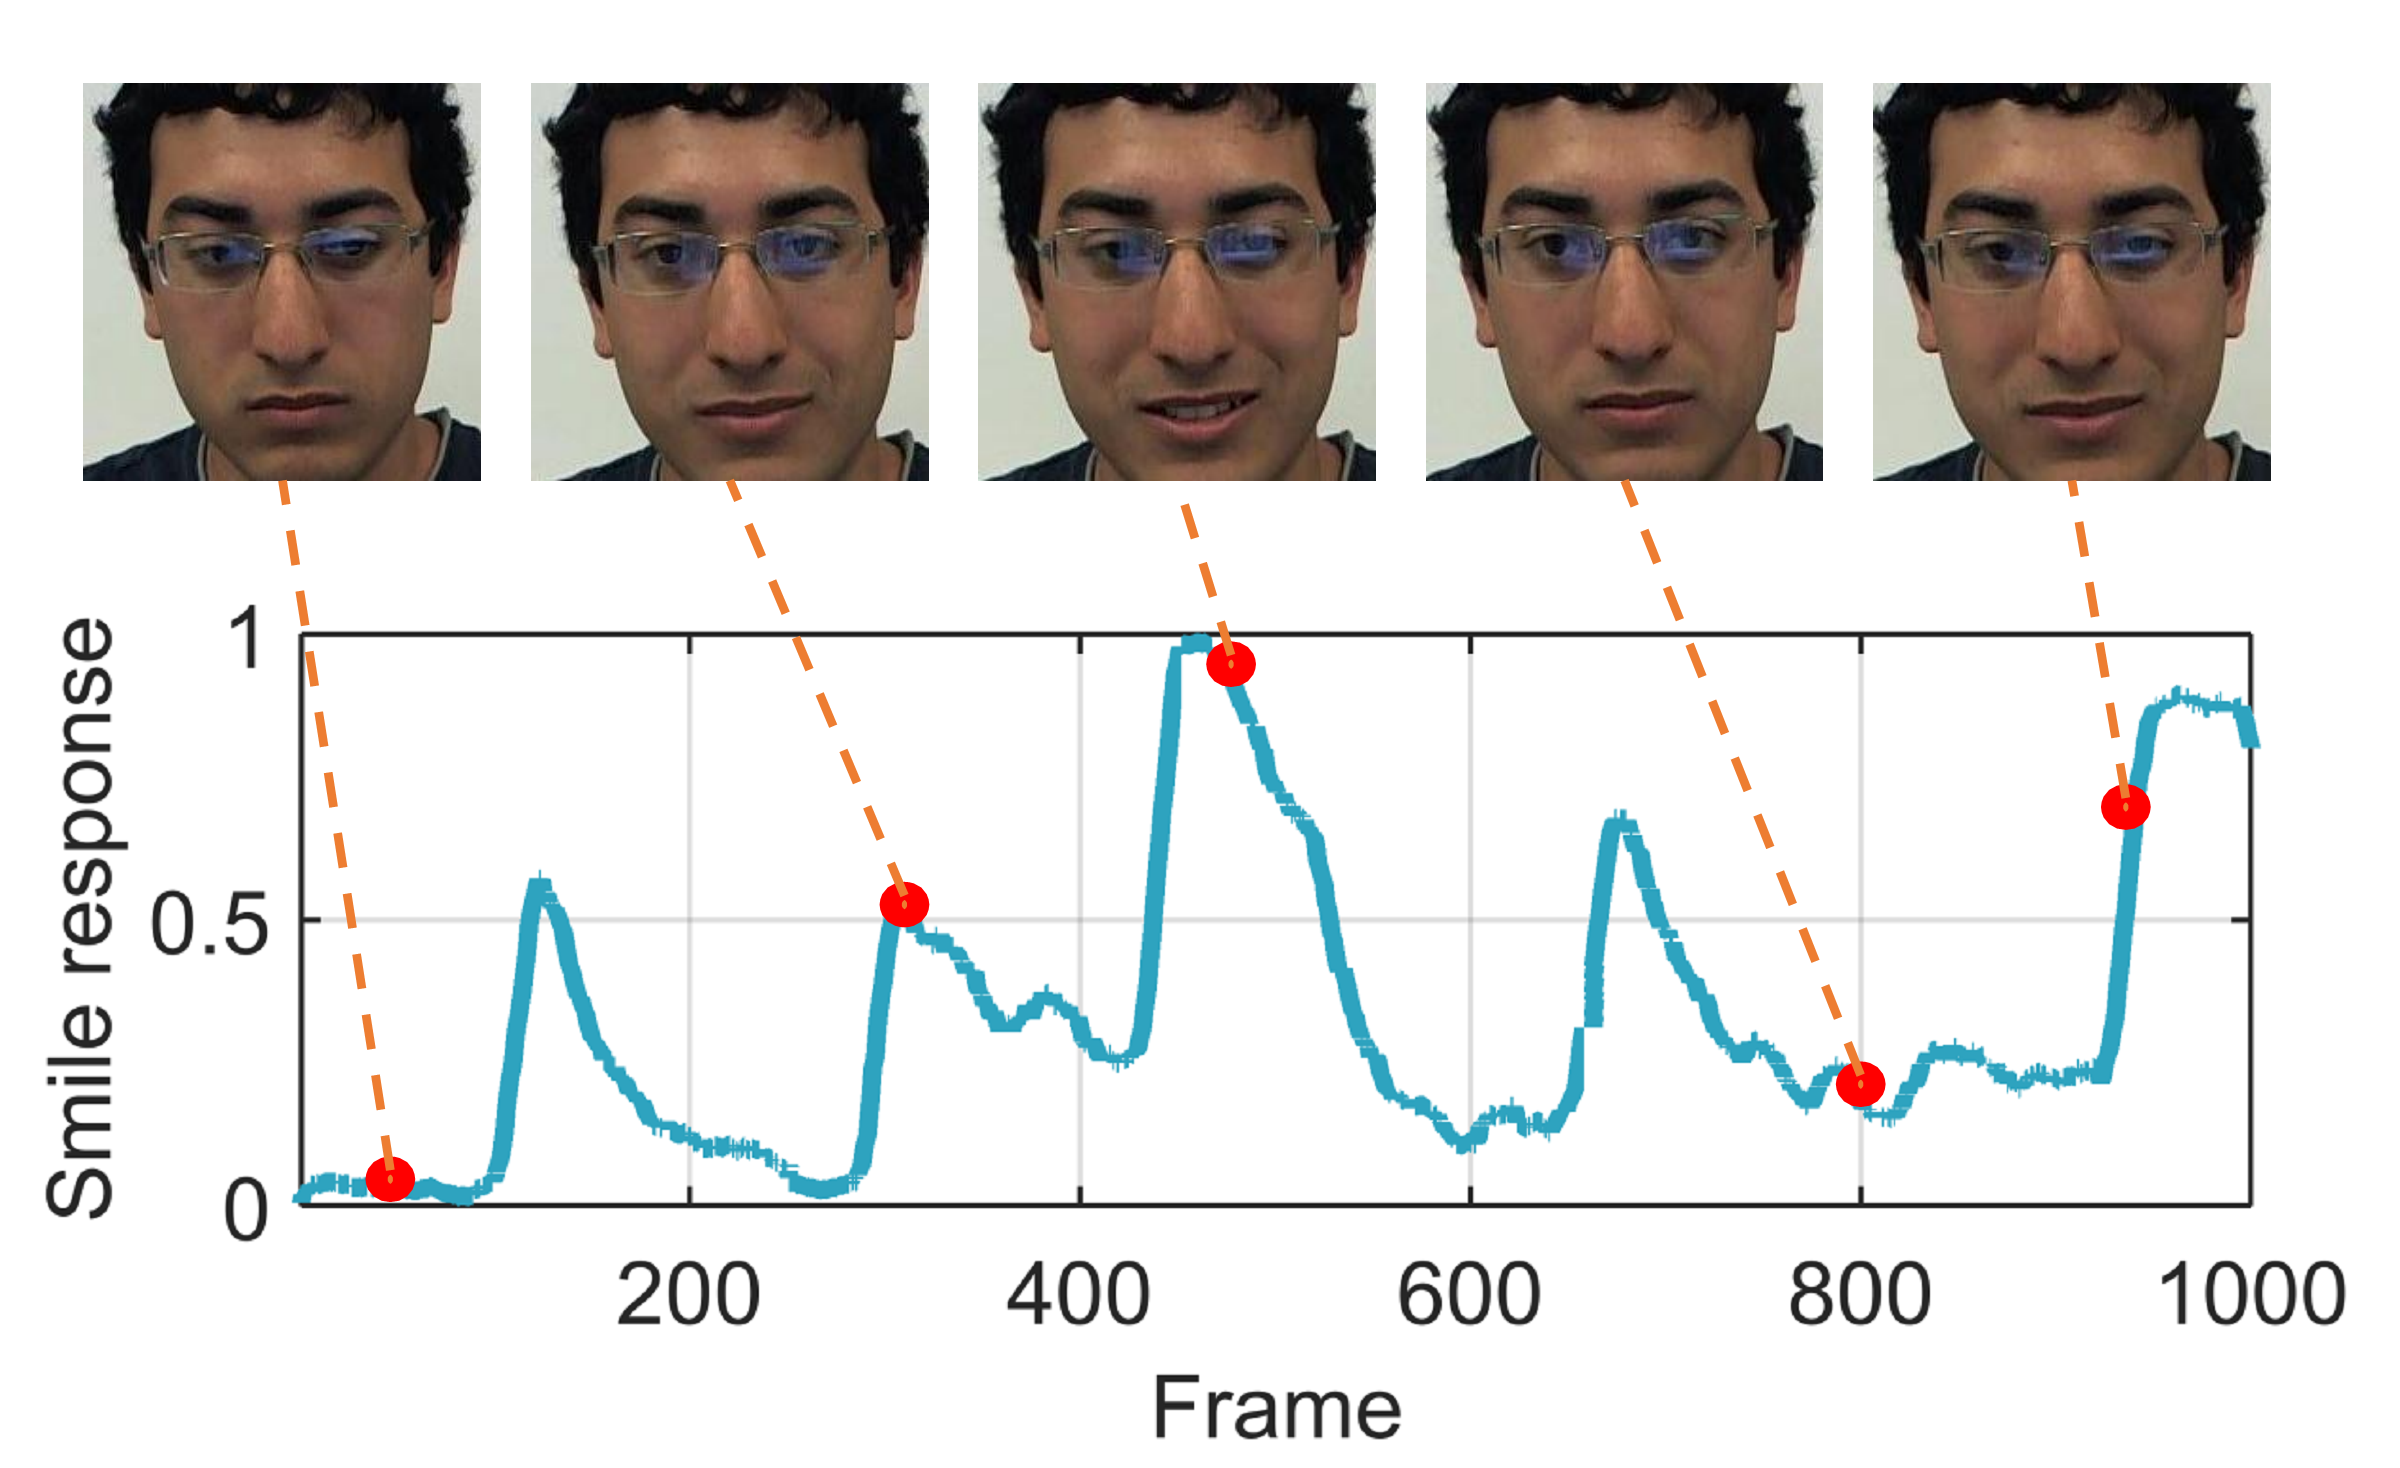
\includegraphics[width=.8\columnwidth]{fig/smile_seq_non_ex.png}\label{fig:ex_non}}
\caption{Examples of smile responses for zapping and non-zapping behavior. For the case of non-zapping, smile response intensity and dynamics are quite distinctive compared to the zapping case.}
\label{fig:smile_ex}
\end{figure}

\subsection{Smile Intensity Estimation.}

\SFAdd{To predict zapping behavior from smile response, we first explain how we estimate the smile intensity on a per frame basis.} \Songfan{The faces are first extracted using Viola-Jones face detector~\cite{Viola_IJCV04}. We then follow our previous work~\cite{Yang13} to align the faces using dense flow-based similarity registration technique. This registration algorithm aligns every frame with a face to a reference face and the registration results are temporally smoothed. Thus, the person-independent spontaneous facial expression recognition can be carried out in a meaningful manner. The aligned faces which are scaled to $200\times200$ pixels, are divided into $20\times20$ pixel regions. The Local Phase Quantization~\cite{Ojansivu_ICISP08} texture descriptor is computed for each of the regions. These outputs are then concatenated to form the feature for smile detection.}

\Songfan{The smile detection is formulated as a binary classification problem with the smiling face and neutral face being the two class labels. We adopt the linear SVM~\cite{SVMlib} for classification. For accurate person-independent smile detection, the classifier is trained on multiple databases with a large number of subjects from: FEI~\cite{FEI}, Multi-PIE~\cite{MPIE}, CAS-PEAL~\cite{CAS}, CK+~\cite{CKplus}, and data from Google image search similar to~\cite{Le14}. In total, 1543 subjects (1543 smiling faces and 2035 neutral faces) are included for training. }

\begin{figure}[htbp]
\centering
    \subfigure[Training data]{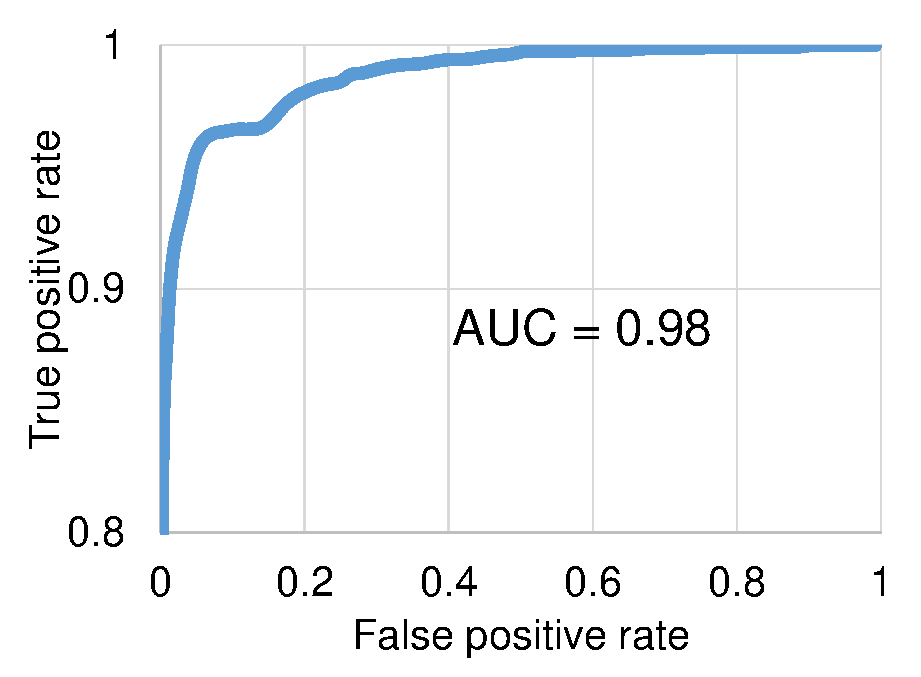
\includegraphics[width=.46\columnwidth]{fig/smile_roc_train.eps}\label{fig:smile_roc_train}}
    \subfigure[Testing data]{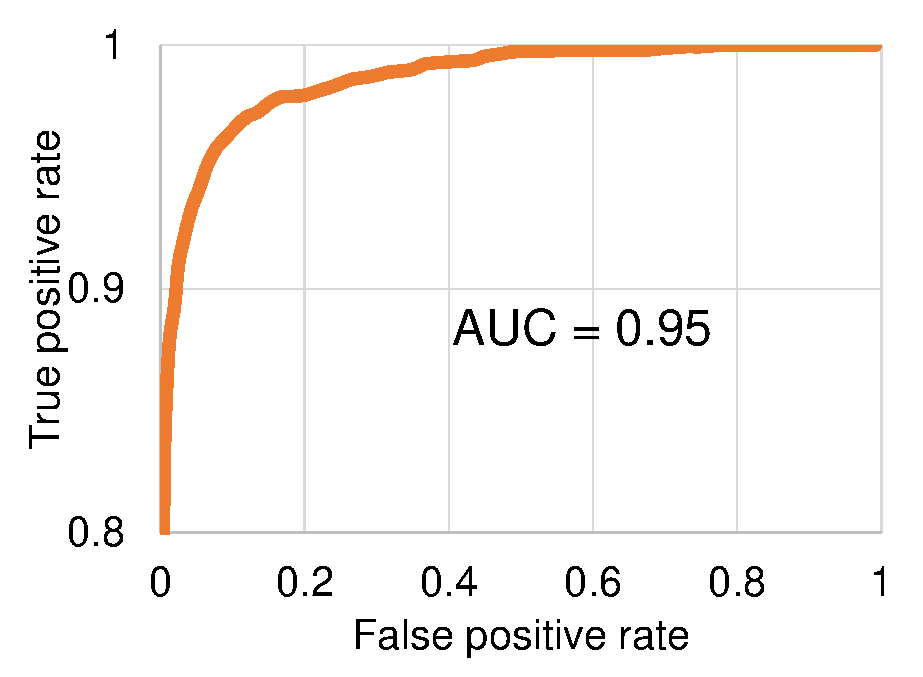
\includegraphics[width=.46\columnwidth]{fig/smile_roc_test.eps}\label{fig:smile_roc_test}}

\caption{Classification results of our person-independent smile detection approach shown by ROC curves.}
\end{figure}


\Songfan{A series of tests are carried out in a person-independent manner where no test subject is included during training. The Area Under Curve (AUC) is 0.98 for the 10-fold cross validation (see Fig.~\ref{fig:smile_roc_train}). To demonstrate the generalization of this classifier, we carried out a test on a selection of 10,000 sample frames from our aforementioned database that we collected in this research. The Area Under Curve (AUC) is 0.95 in Fig.~\ref{fig:smile_roc_test}, which means that the smile classifier performs well on unseen data. The probability output of the SVM smile classifier is then recorded as the smile response. We direct interested readers to~\cite{Yang_TAC14} for a more detailed validation on why smile intensity estimation is correlated with the SVM probability output.}


\section{Methodology}%: Responselet Dictionary Learning}
To predict MMZP given smile responses, we formulated it as a zapping vs. non-zapping binary classification problem on a per frame basis. Below we explain in detail how zapping is quantified and how the features are extracted to predict zapping.

%During the training phase, a \textit{responselet} dictionary is learnt from the time series of facial responses. This dictionary consists of the basis to reconstruct the entire smile response signal. During testing, a local responselet is sparsely reconstructed from the learnt dictionary and the reconstruction coefficients are used as features for prediction. \textit{We treat the probability prediction as the representation of our MMZP. ??? } Details of the methodology are presented in the following.

\subsection{Zapping Quantification.}

Since the subjects are given the option to zap at any time, the fraction of an ad being watched varies for different participants. Fig.~\ref{fig:ad_len_distr} shows the distribution of ad fraction that is being watched. It can be observed that most ads have been watched at least 80\% of their length. Besides, participants in our experiments tended to zap early if they are not attracted to an ad, as evidenced by the left part of the plot (i.e., 0\% to 30\% has a slightly higher probability). To distinguish zapped and non-zapped cases, a Gaussian mixture model with three components is fitted to the data. As seen in Fig.~\ref{fig:ad_len_distr}, the left-most and right-most Gaussian models are with low variance and well capture the distinctiveness of zapping and non-zapping class, respectively. The Gaussian model in the middle with high variance includes the sequences that are on the boundary of two classes. As a result, we empirically select the mean of the second mixture, 0.56, as the threshold to distinguish zapping from non-zapping sequences.

\begin{figure}[h]
	\centering
		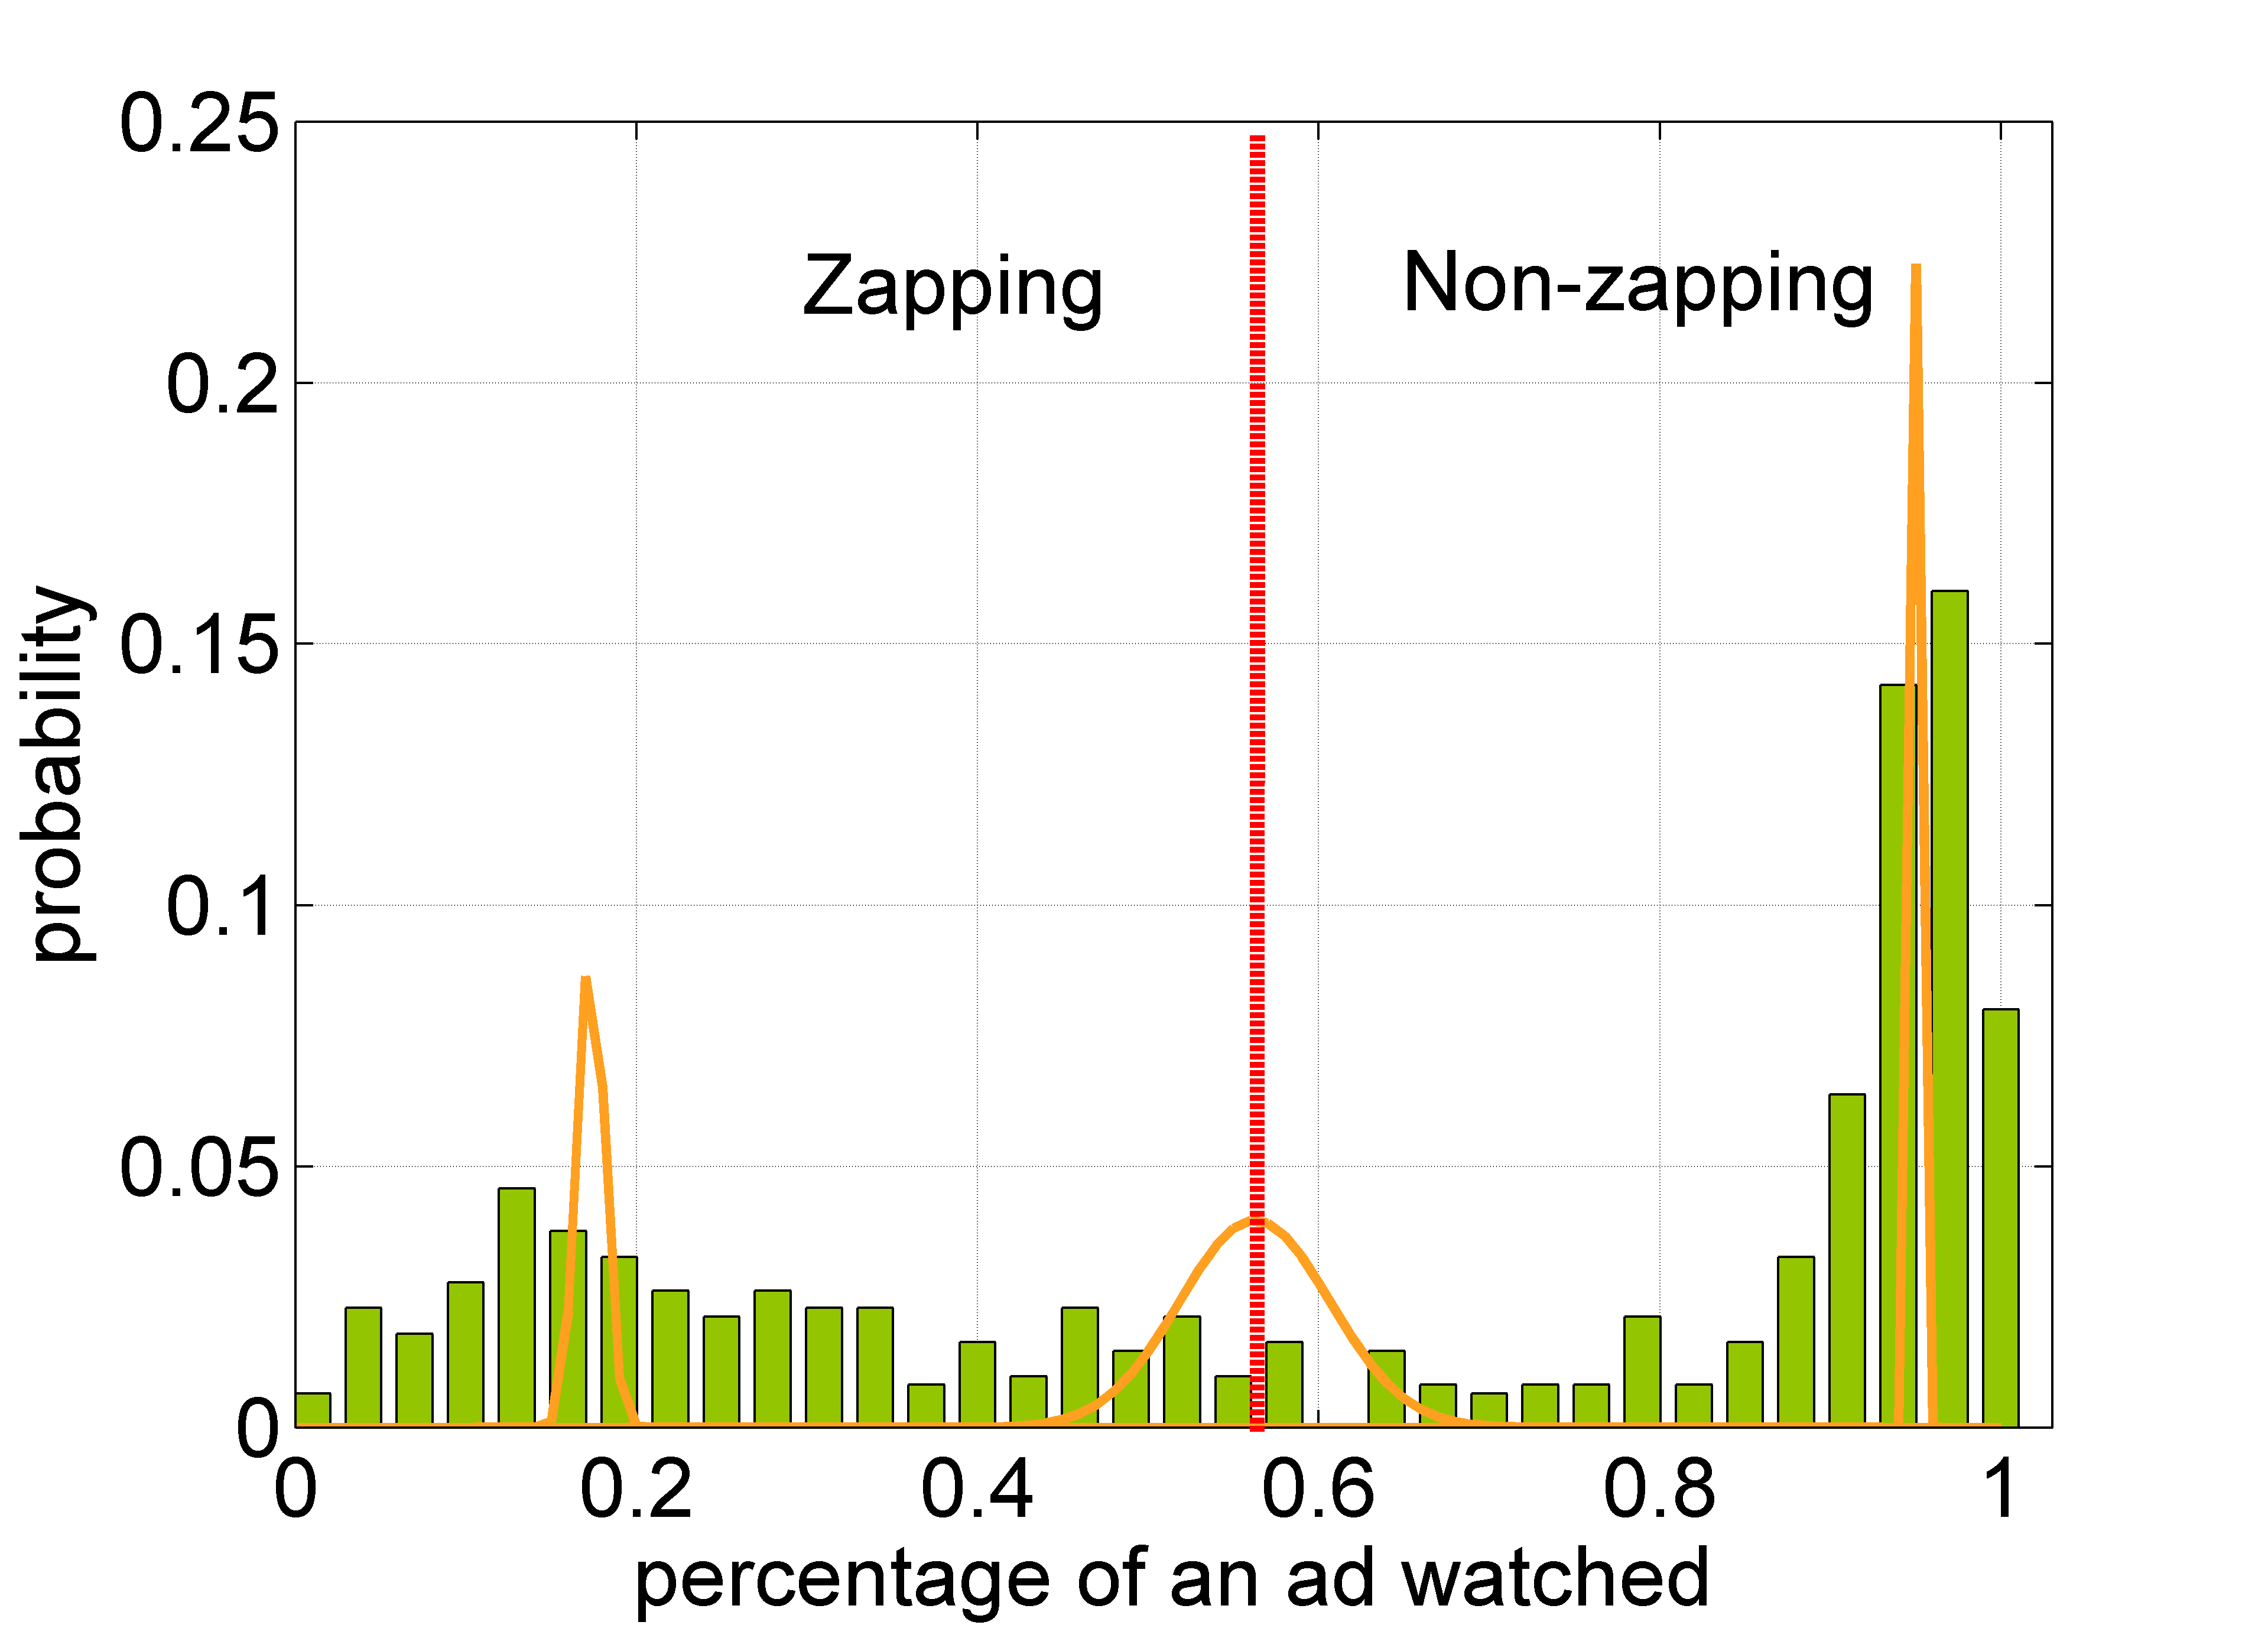
\includegraphics[width=.85\columnwidth]{fig/ad_len_distr.png}
	\caption{The zapping distribution. We use Gaussian mixture model to fit the data. The left-most and right-most Gaussians well capture the distinctiveness of zapping and non-zapping classes, respectively. The middle Gaussian with high variance represents the sequences that are on the boundary of two classes. We use the mean of the second Gaussian, 0.56, as a data-driven threshold to distinguish zapping from non-zapping.}
	\label{fig:ad_len_distr}
\end{figure}

\subsection{Zapping Prediction.}

During the training phase, a dictionary of \textit{responselet} (i.e., small segments of smile response) is learned from the recorded subjects' facial responses. Then given a smile responselet, it is first reconstructed by the learned dictionary and the reconstruction coefficients are used as features to train a zapping prediction model. During testing, reconstruction coefficients for a responselet is used for zapping prediction with the trained model. 

\noindent \textbf{Responselet Dictionary Learning.} The history of the dictionary design can be traced back to the fast Fourier transform (FFT) or wavelets. In recently years, dictionary learning for sparse representation has prevailed in signal processing and computer vision tasks. In our case, we learn the dictionary which can well reconstruct the input signal in a sparse manner. 

Concretely, \SFAdd{a smile responselet is defined as a 1-D time series data of length $m$, whose value ranges from 0 to 1}; given a set of $n$ smile responselet, $\X=[\x_1, \cdots, \x_n]\in \mathcal{R}^{m\times n}$, a dictionary $\D=[d_1,\cdots,d_p] \in \mathcal{R}^{m\times p}$ is learned by minimizing

\begin{align}
\label{eq:learn_dict}
\min_{\D , \alpha} \sum_{i=1}^n ||\x_i-\D\alpha_i||^2_2 +\lambda ||\alpha_i||_1,
\end{align}

\noindent where $\forall j=1,\cdots,k, d^\top_j d_j \leq 1$. $\lambda$ is a regularization parameter to control the sparsity on $\alpha$. Eq.~(\ref{eq:learn_dict}) can be efficiently solved by an online optimization algorithm~\cite{spams}. 

Consider a subject watching an ad as one data sequence, with 51 subjects and 8 ads, there are 408 sequences. As seen in Fig.~\ref{fig:smile_ex}, the dynamics of the smile response has different lengths. Therefore, each sequence is normalized to 100 frames and each responselet contains 10 frames and the stride of the moving window for the next responselet is set to 1. A dictionary with $p=36$ responselet atoms is learned and visualized in Fig.~\ref{fig:dict} with atoms sorted by their absolute gradient variance. 

\begin{figure}[h]
	\centering
		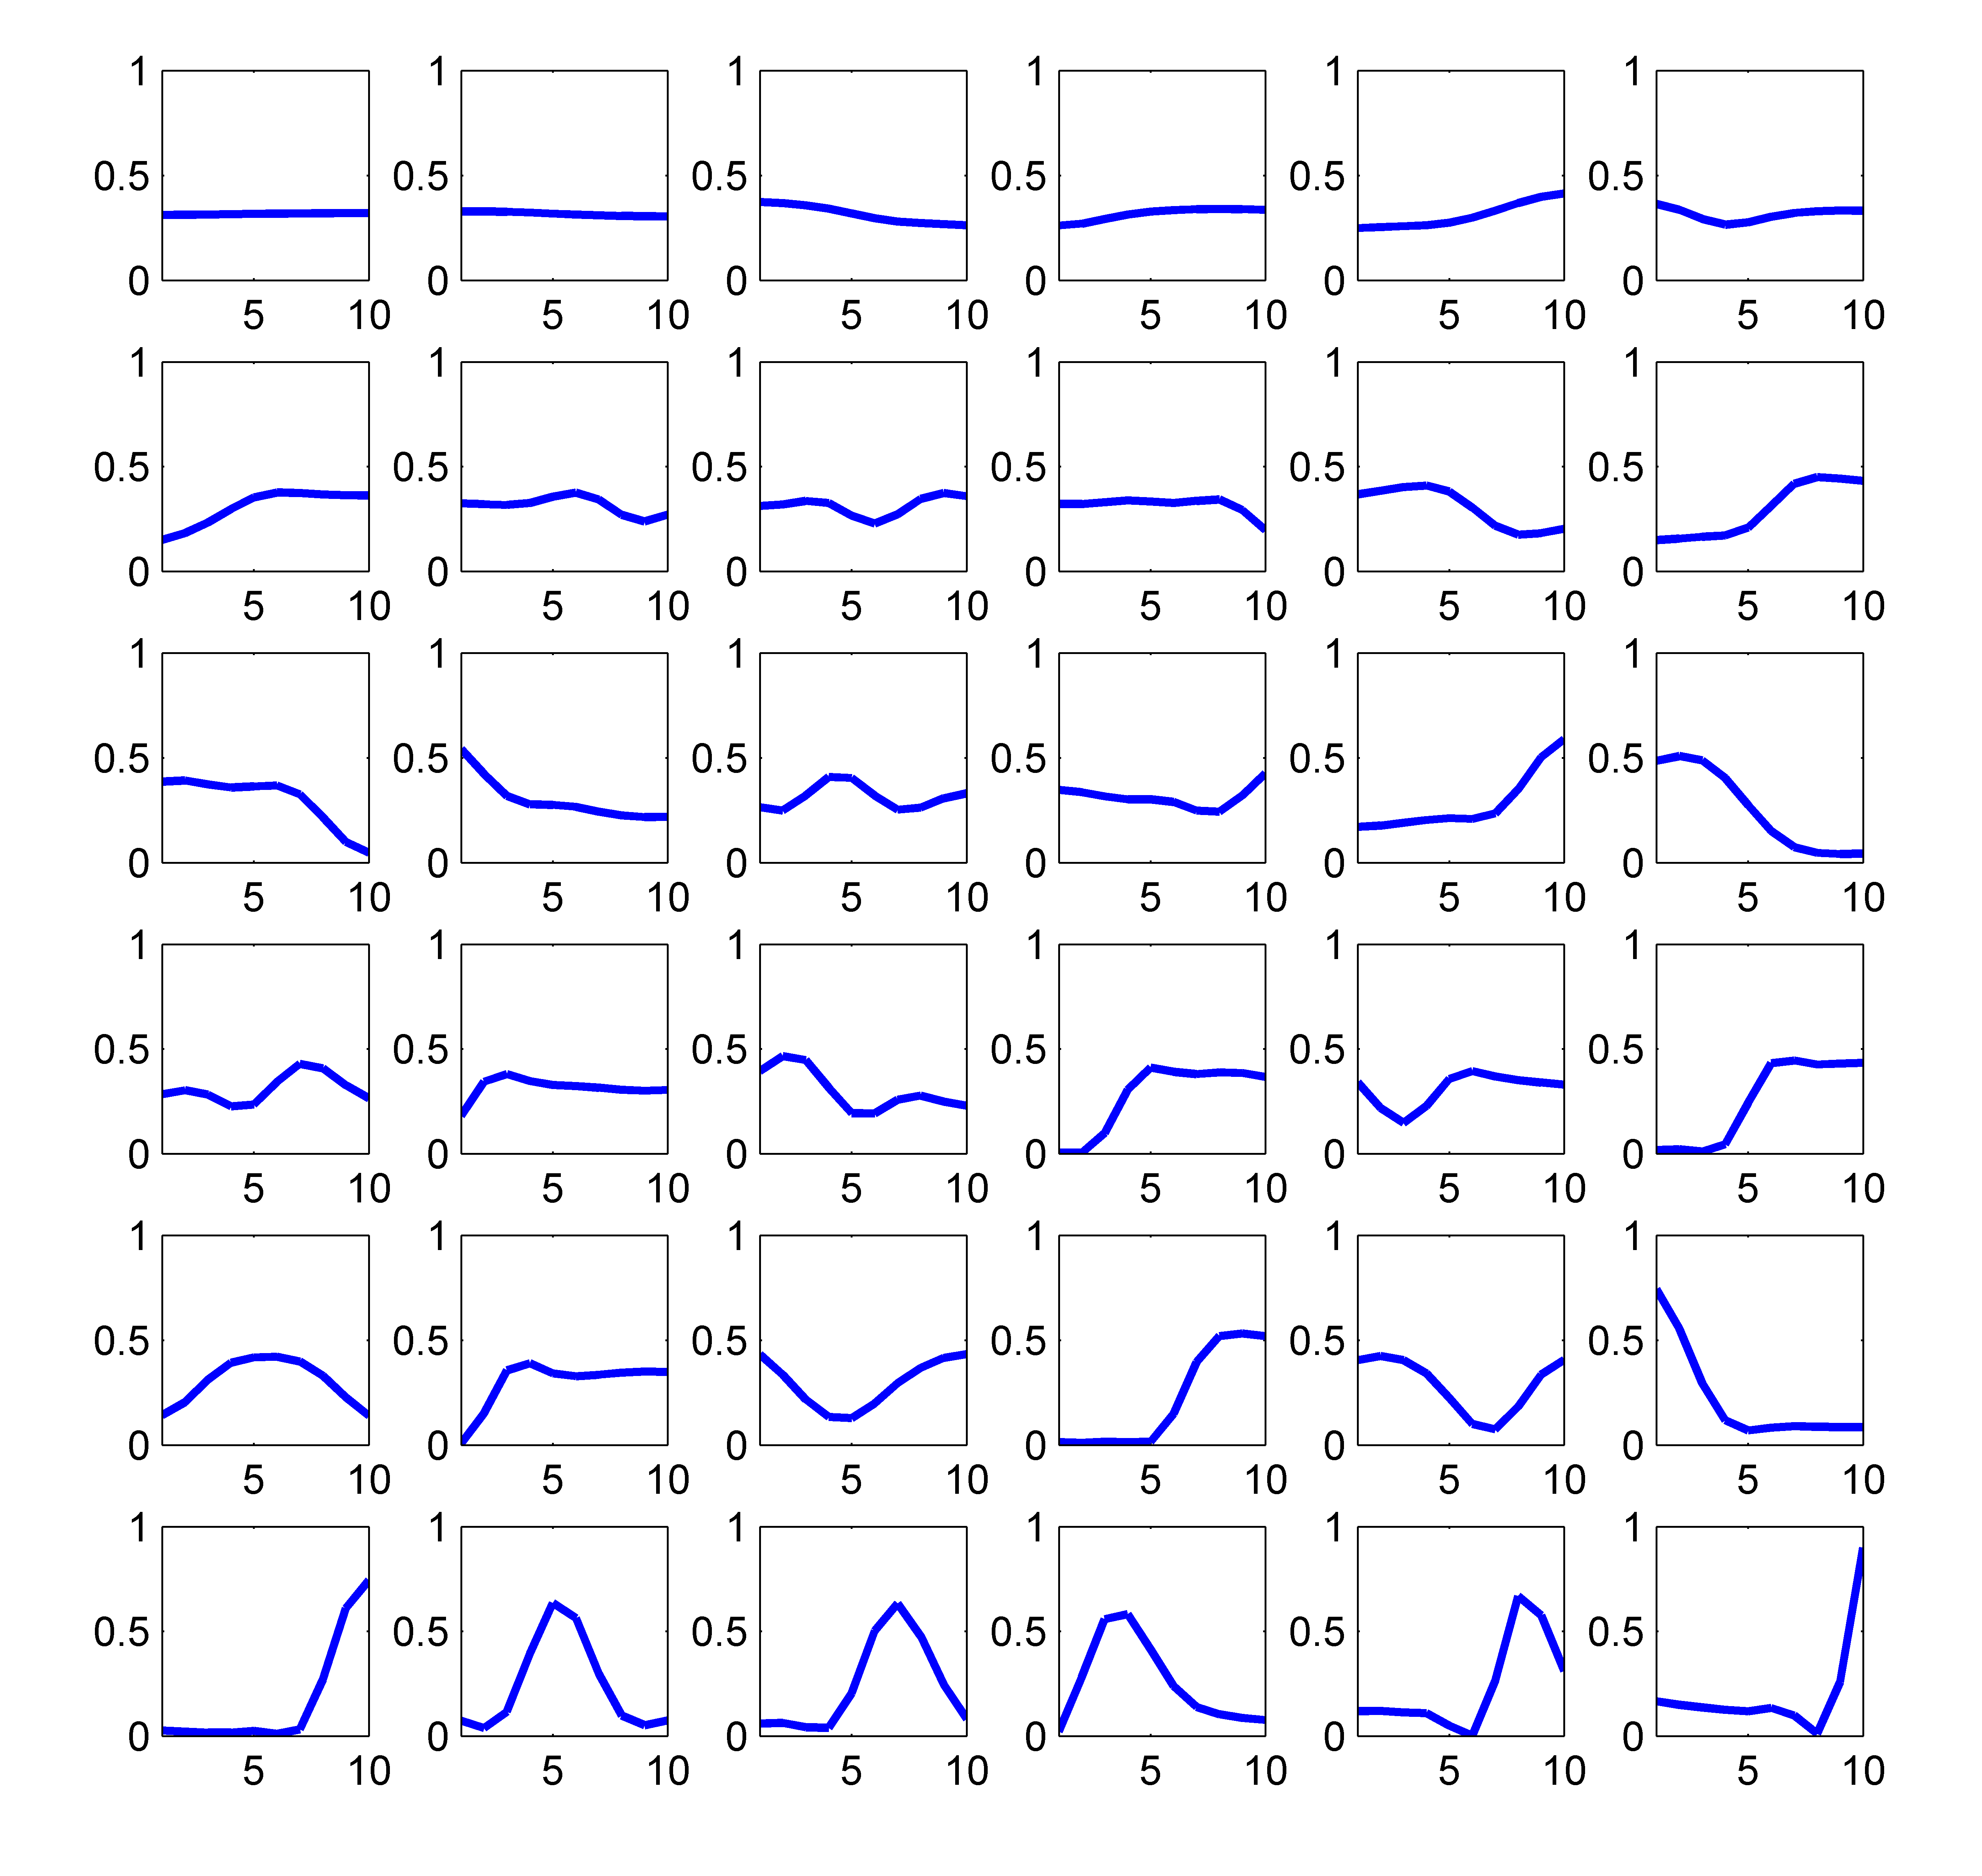
\includegraphics[width=1\columnwidth]{fig/dict.png}
	\caption{The learned responselet dictionary.}
	\label{fig:dict}
\end{figure}

\begin{figure}[h]
	\centering
		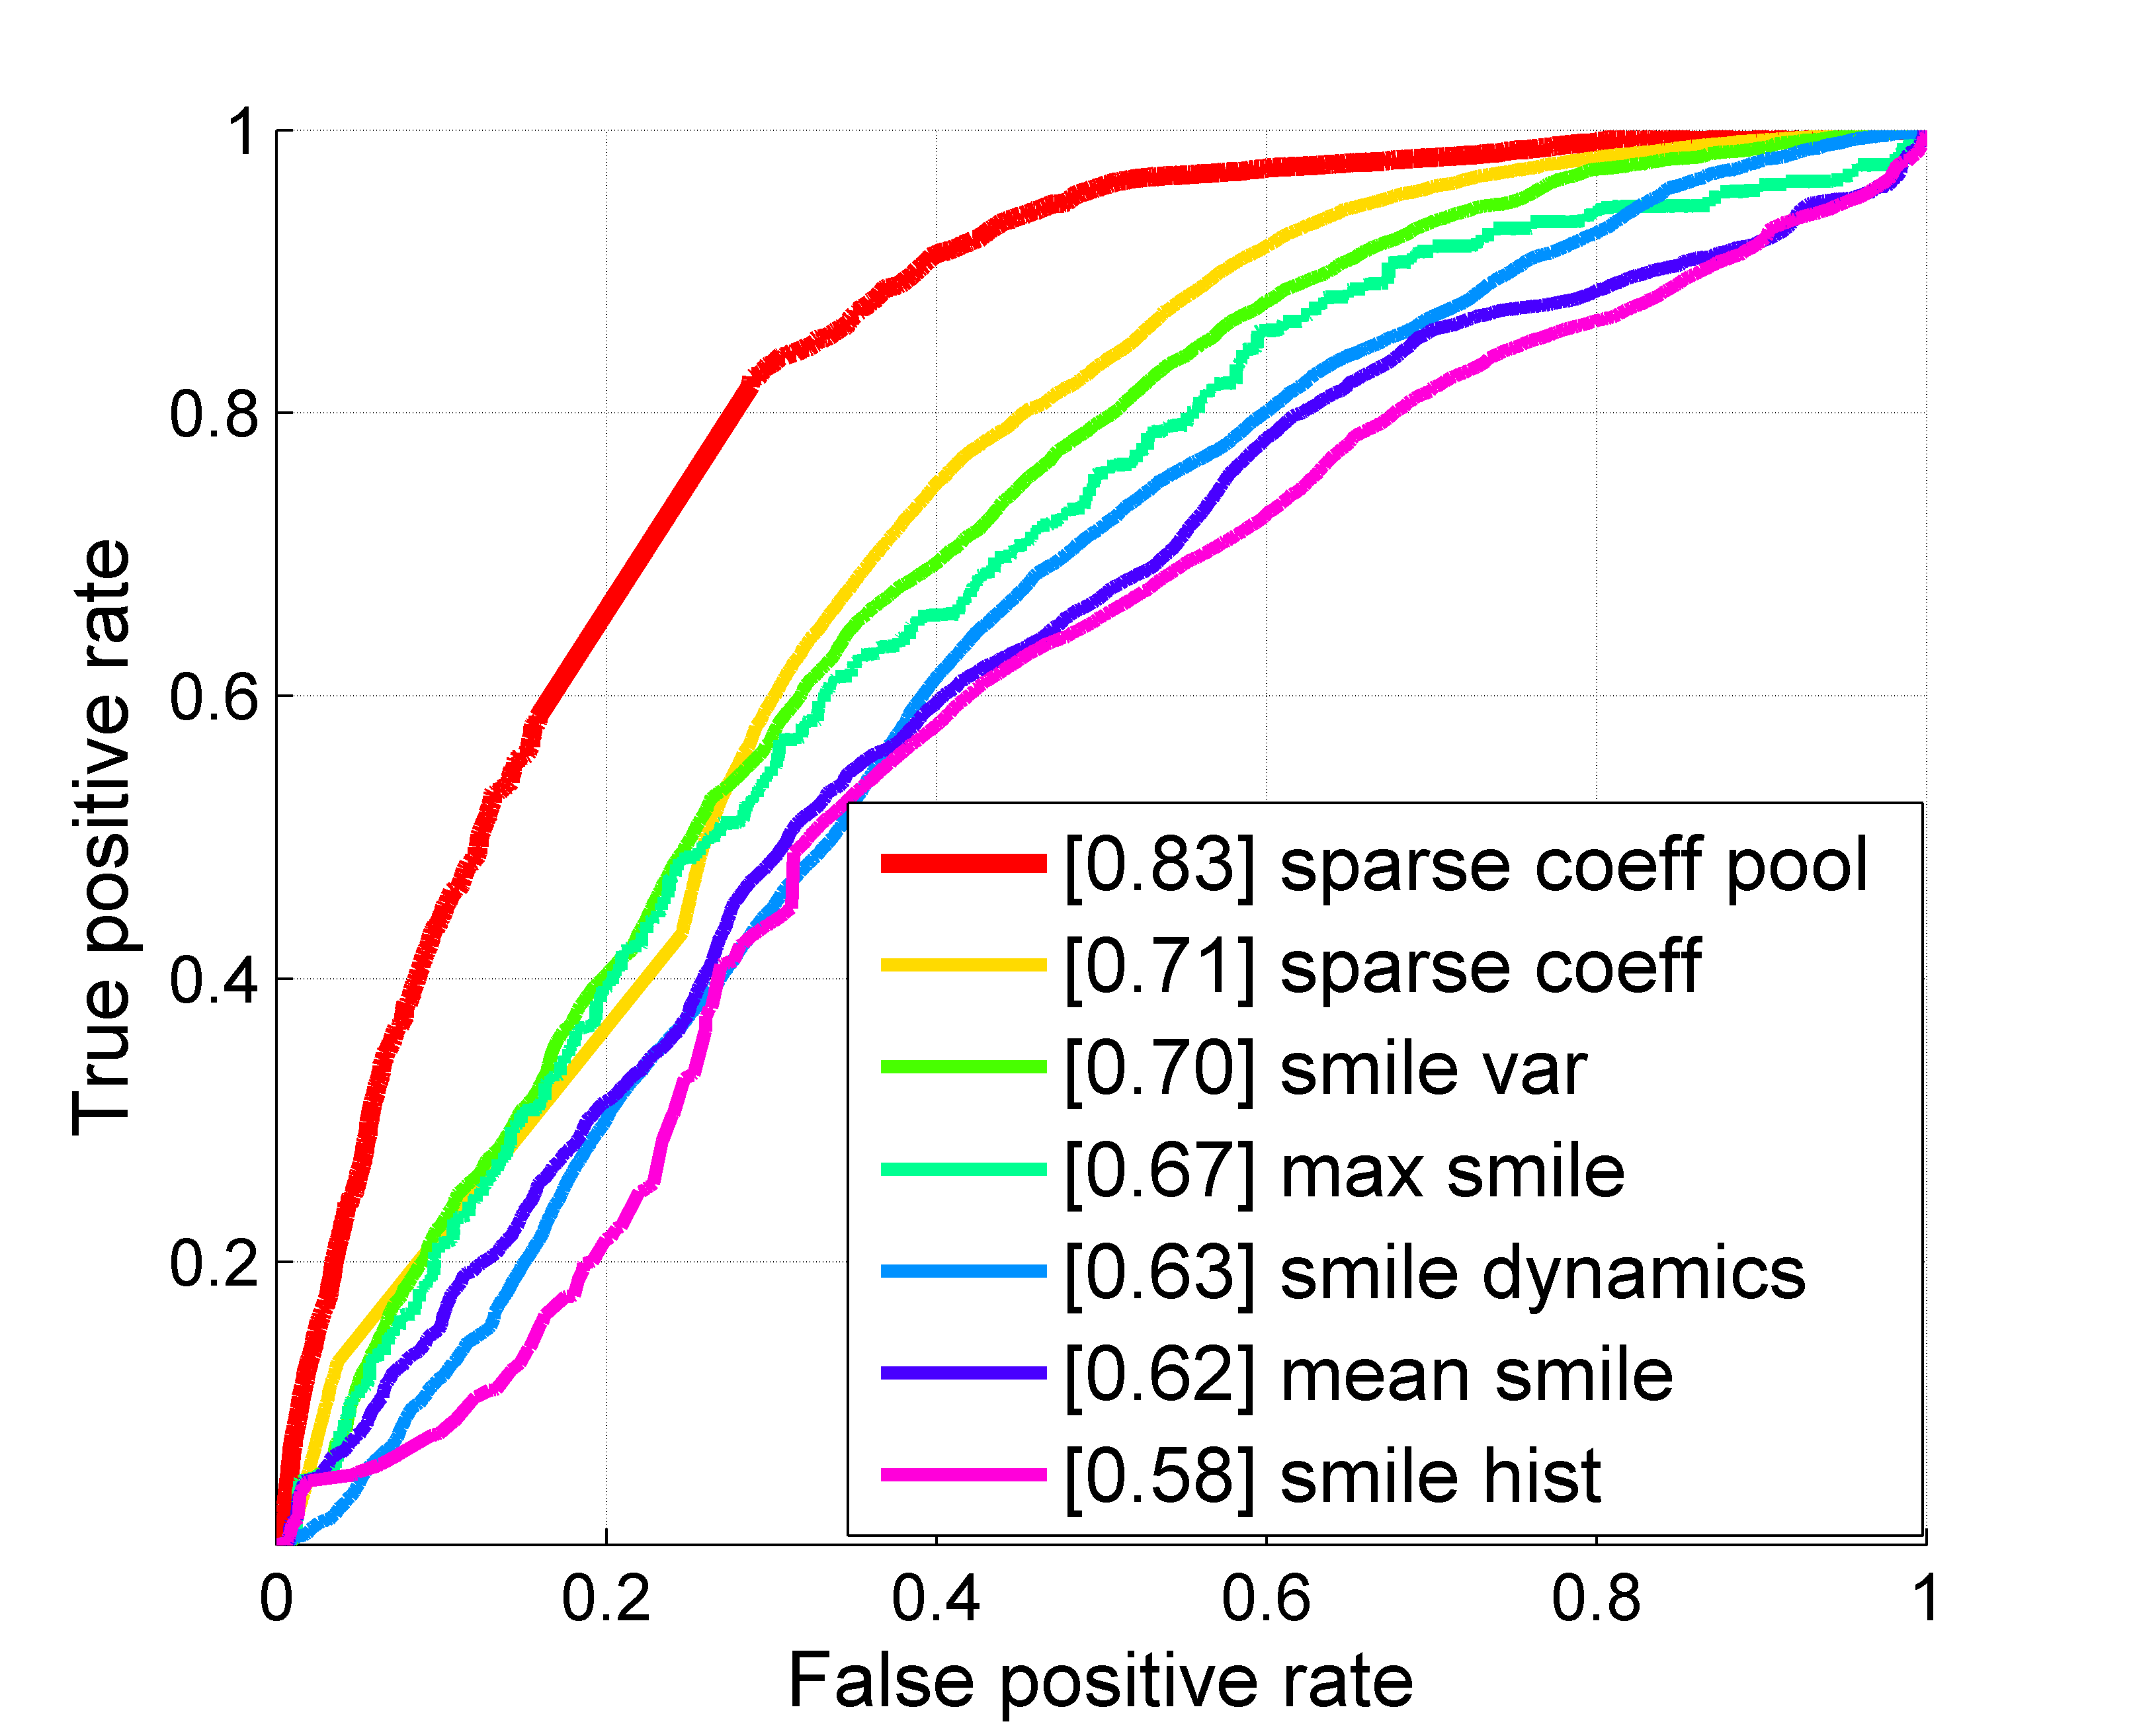
\includegraphics[width=.85\columnwidth]{fig/cls_performance.png}
	\caption{The ROC curves for zapping classification using various features. Numbers are the area under the curve (AUC) values.}
	\label{fig:cls_performance}
\end{figure}


\begin{figure*}[t]
	\centering
		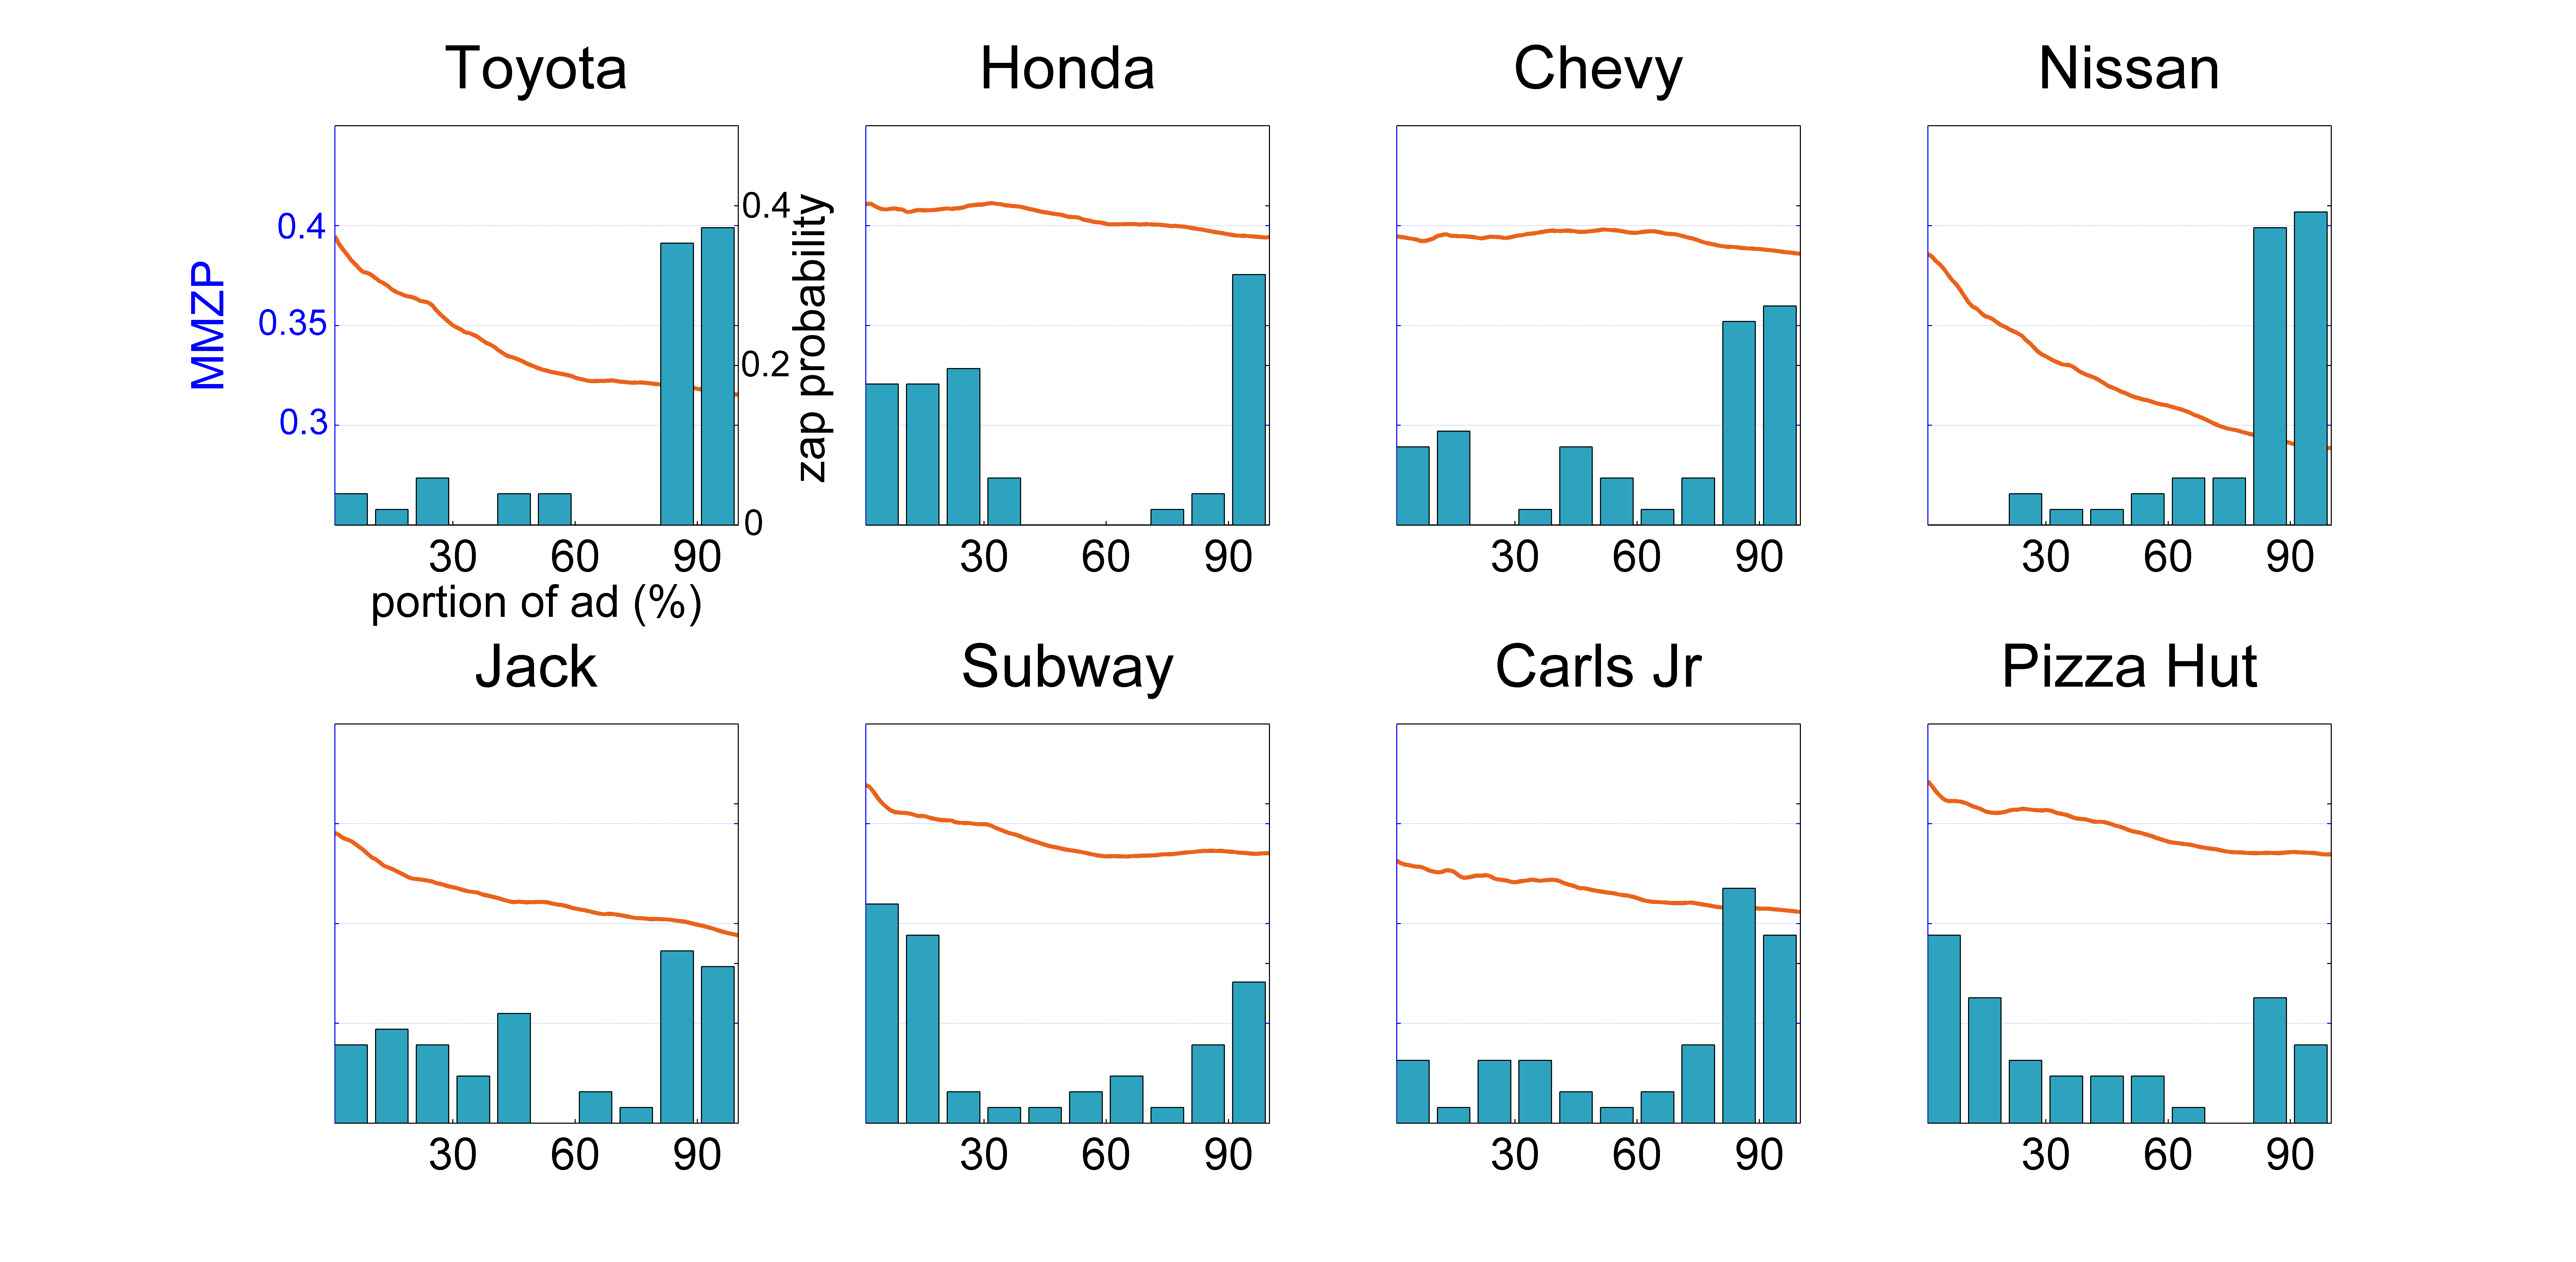
\includegraphics[width=.8\textwidth]{fig/ad.png}
	\caption{MMZP of different ads. The lines show the MMZP trends and the bars show the corresponding ground truth zapping distribution. The axis and labels are the same across all sub-figures and are displayed in the first panel only for compactness. We use the same display settings for the rest of the figures.}
	\label{fig:ad}
\end{figure*}

As seen in Fig.~\ref{fig:dict}, the learned dictionary atoms start from flat shape (upper left), gradually vary in slope, and finally transform to bell shapes representing much more fine-grained changes (bottom two rows). The expressiveness of the learned dictionary ensures that a new responselet can be well represented. 


\noindent \textbf{Training of Zapping Prediction Model.} Having learned the dictionary $\D$, at each frame, say $k$, we first divide the response from frame 1 to $k$ into $k-10+1$ number of responselets (i.e., 10 frames per responselets) with a stride of one frame in the same way as aforementioned. Then, these responselets are sparsely reconstructed by $\D$ using Eq.~(\ref{eq:learn_dict}) with $\D$ fixed. Thus, for each responselet, we obtain a $p\times 1$ reconstruction coefficient vector. To encode the between frame information, we perform mean-pooling of all available coefficient vectors for the responselets generated from frame 1 to $k$, yielding our final feature representation of size $p\times 1$. Features extracted from training data are then used to learn a linear SVM classifier to predict zapping at each moment (i.e., each frame).

\noindent \textbf{Testing of Zapping Prediction Model.} The zapping prediction model is evaluated using leave-one-subject-out cross validation. In each fold, one subject is held out for testing, and the others are used for training. Besides mean-pooled features, we have also included several other features as baselines for comparison,  including: mean, max, variance of smile response, smile dynamics (meaning that we directly use the length-normalized smile response as features), and smile histogram~\cite{Yang_TAC14}. In addition, we also compare with direct use of the sparse reconstruction coefficients without mean-pooling.

As shown in Fig.~\ref{fig:cls_performance}, sparse coefficients with mean-pooling significantly outperforms the other features. This is attributed to the fact that mean-pooling takes into the account the between-frame information and yields a more stable representation than other features. Smile variance performs slightly better than other smile response variants. This also demonstrates that the shape of a smile response is discriminative to distinguish zapping from non-zapping. 



\section{Knowledge Discovery}

As aforementioned, MMZP represents the dynamics of users' interest level while watching an ad. In general, increased MMZP correlates with more chances of zapping due to lack of interest in the ad content. To validate this conclusion, we first examine the effectiveness of MMZP, and then provide a series of knowledge discovery from the observations on MMZP changes. 

\noindent \textbf{MMZP Validation.} To validate the accuracy of MMZP, we first compare it with the actual user zapping behavior. In Fig.~\ref{fig:ad}, the mean MMZP (left axis) of all subjects for each ad is plotted and is compared with the ground truth zapping behavior as shown in the bar plot of each panel (right axis). Note that the zapping behavior is represented by the percentage of an ad being watched, which was recorded during data collection. In general, the fast decreasing pattern of MMZP (less likely to zap) correlates with zapping behavior occurring near the end of an ad (e.g., \textit{Toyota} and \textit{Nissan}). In other words, zapping near the end suggests that more interesting contents in the ad were found by the user. On the other hand, slowly decreasing or stable MMZP indicates more chances of zapping (e.g., \textit{Chevy} and \textit{Pizza Hut}). This is congruent with both zapping distribution in the bar plot and the ad entertaining level of each ad as listed in Table~\ref{table:ads}. 

\noindent \textbf{Gender Preference for Ads.} We consider both gender groups watching different ads and discover interesting findings illustrated by some examples in Fig.~\ref{fig:ad_gend}. Based on the MMZP changes, it can be observed that: 1) \textit{Females} prefer \textit{Honda}, probably because of the embedded story about family and pet along with gentle background music; 2) \textit{Males} favor \textit{Jack in the Box}, most likely due to the rock music scene in the ad. Similar observations hold for other ads and these findings suggest that during ad design gender preference shall be leveraged for more precise targeting. 

\begin{figure}[h]
	\centering
		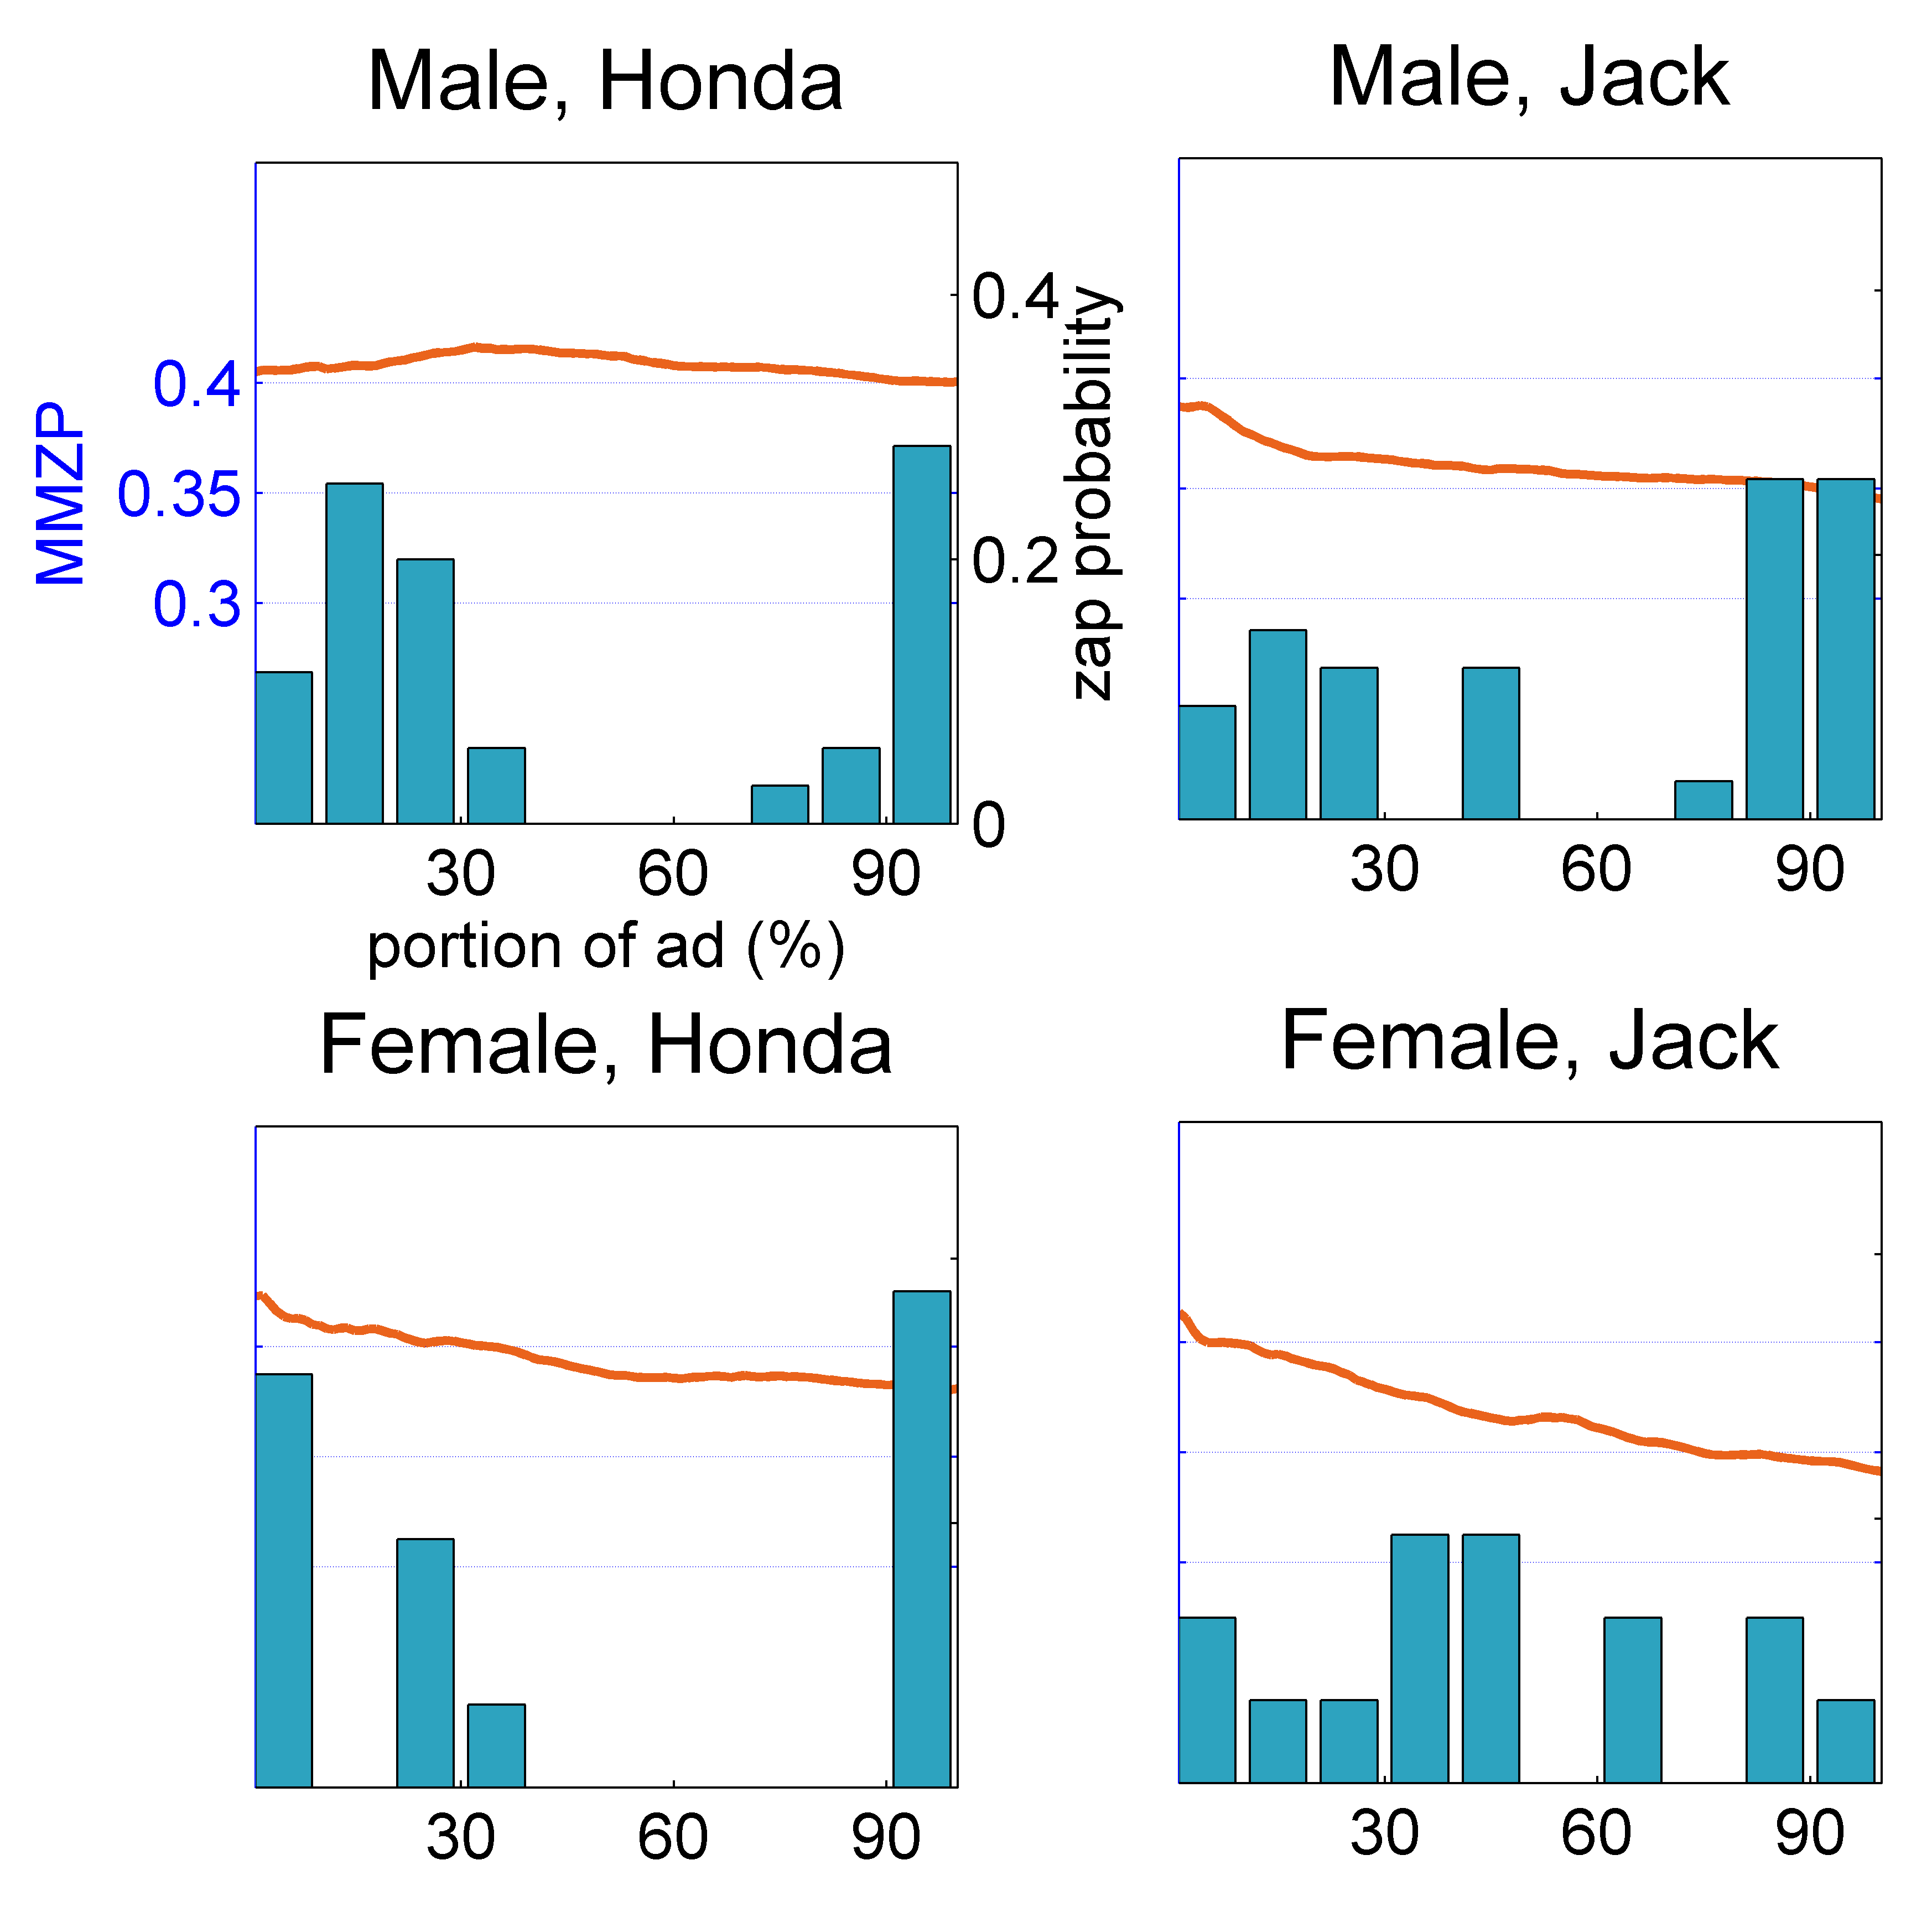
\includegraphics[width=.8\columnwidth]{fig/ad_gend.png}
	\caption{Gender-related ad preference. The \textit{Male} group prefers \textit{Jack in the Box} in which rock music scene is shown. The \textit{Female} group enjoys \textit{Honda} more likely due to its family and pet story setting with gentle background music.}
	\label{fig:ad_gend}
\end{figure}

\noindent \textbf{Ethnicity Preference for Ads.} As seen in Fig.~\ref{fig:eth_ad}, \textit{Asians} show less interest in an entertaining \textit{Toyota} ad. We found out that this is because \textit{Toyota} ad's entertaining factor comes from amusing conversations; while some members in the Asian group, who have just come to the US with English not as their first language, did not catch the full meaning of the conversation. Thus, more zapping happens for the \textit{Asian} group. For another example, \textit{Hispanic} group is less interested in a more direct, food scene oriented \textit{Pizza Hut} ad. Our interview with them suggests that most of them retain their ethnic dining habit in which pizza plays a less important role. Such examples indicate that ad preference is related to a user's ethnicity group and taking this into account in ad design and targeting may result in a better ad campaign.


\begin{figure}[t]
	\centering
		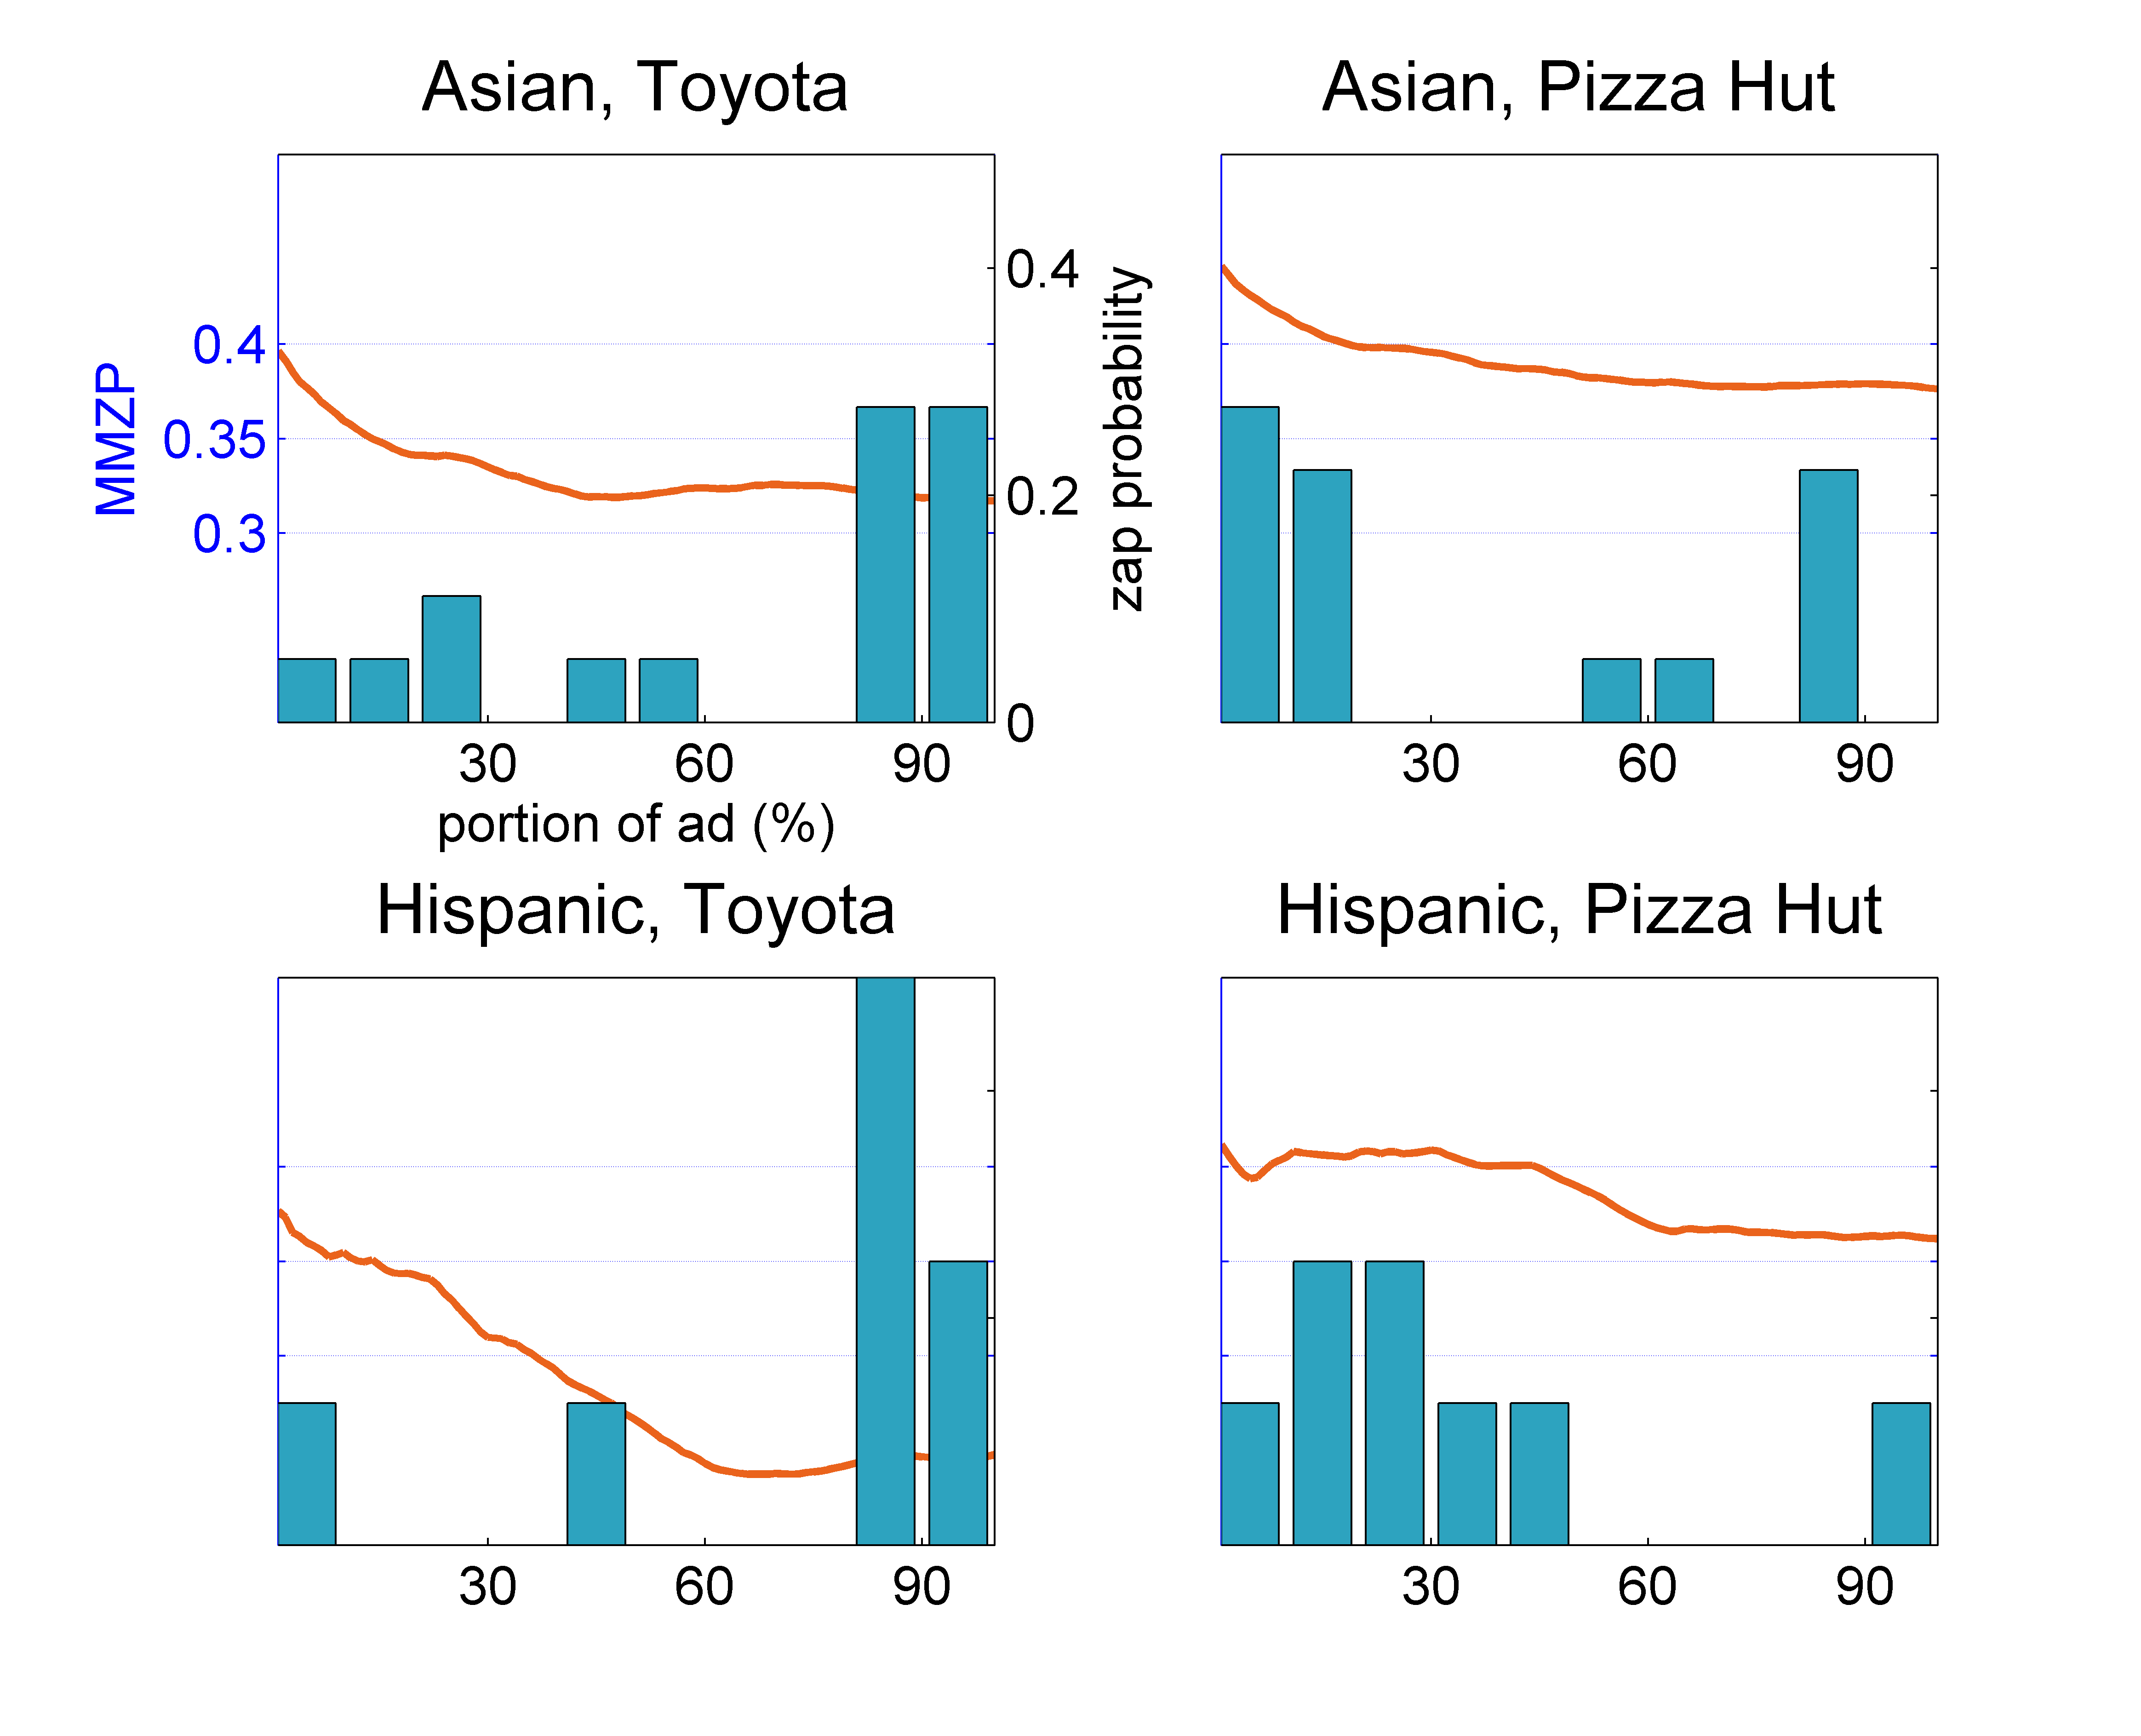
\includegraphics[width=.9\columnwidth]{fig/eth_ad.png}
	\caption{Ethnicity-related ad preference. It is observed that \textit{Asian} group is more likely to zap on \textit{Toyota} while \textit{Hispanic} group does not much enjoy \textit{Pizza Hut}.}
	\label{fig:eth_ad}
\end{figure}

\begin{figure}[t]
	\centering
		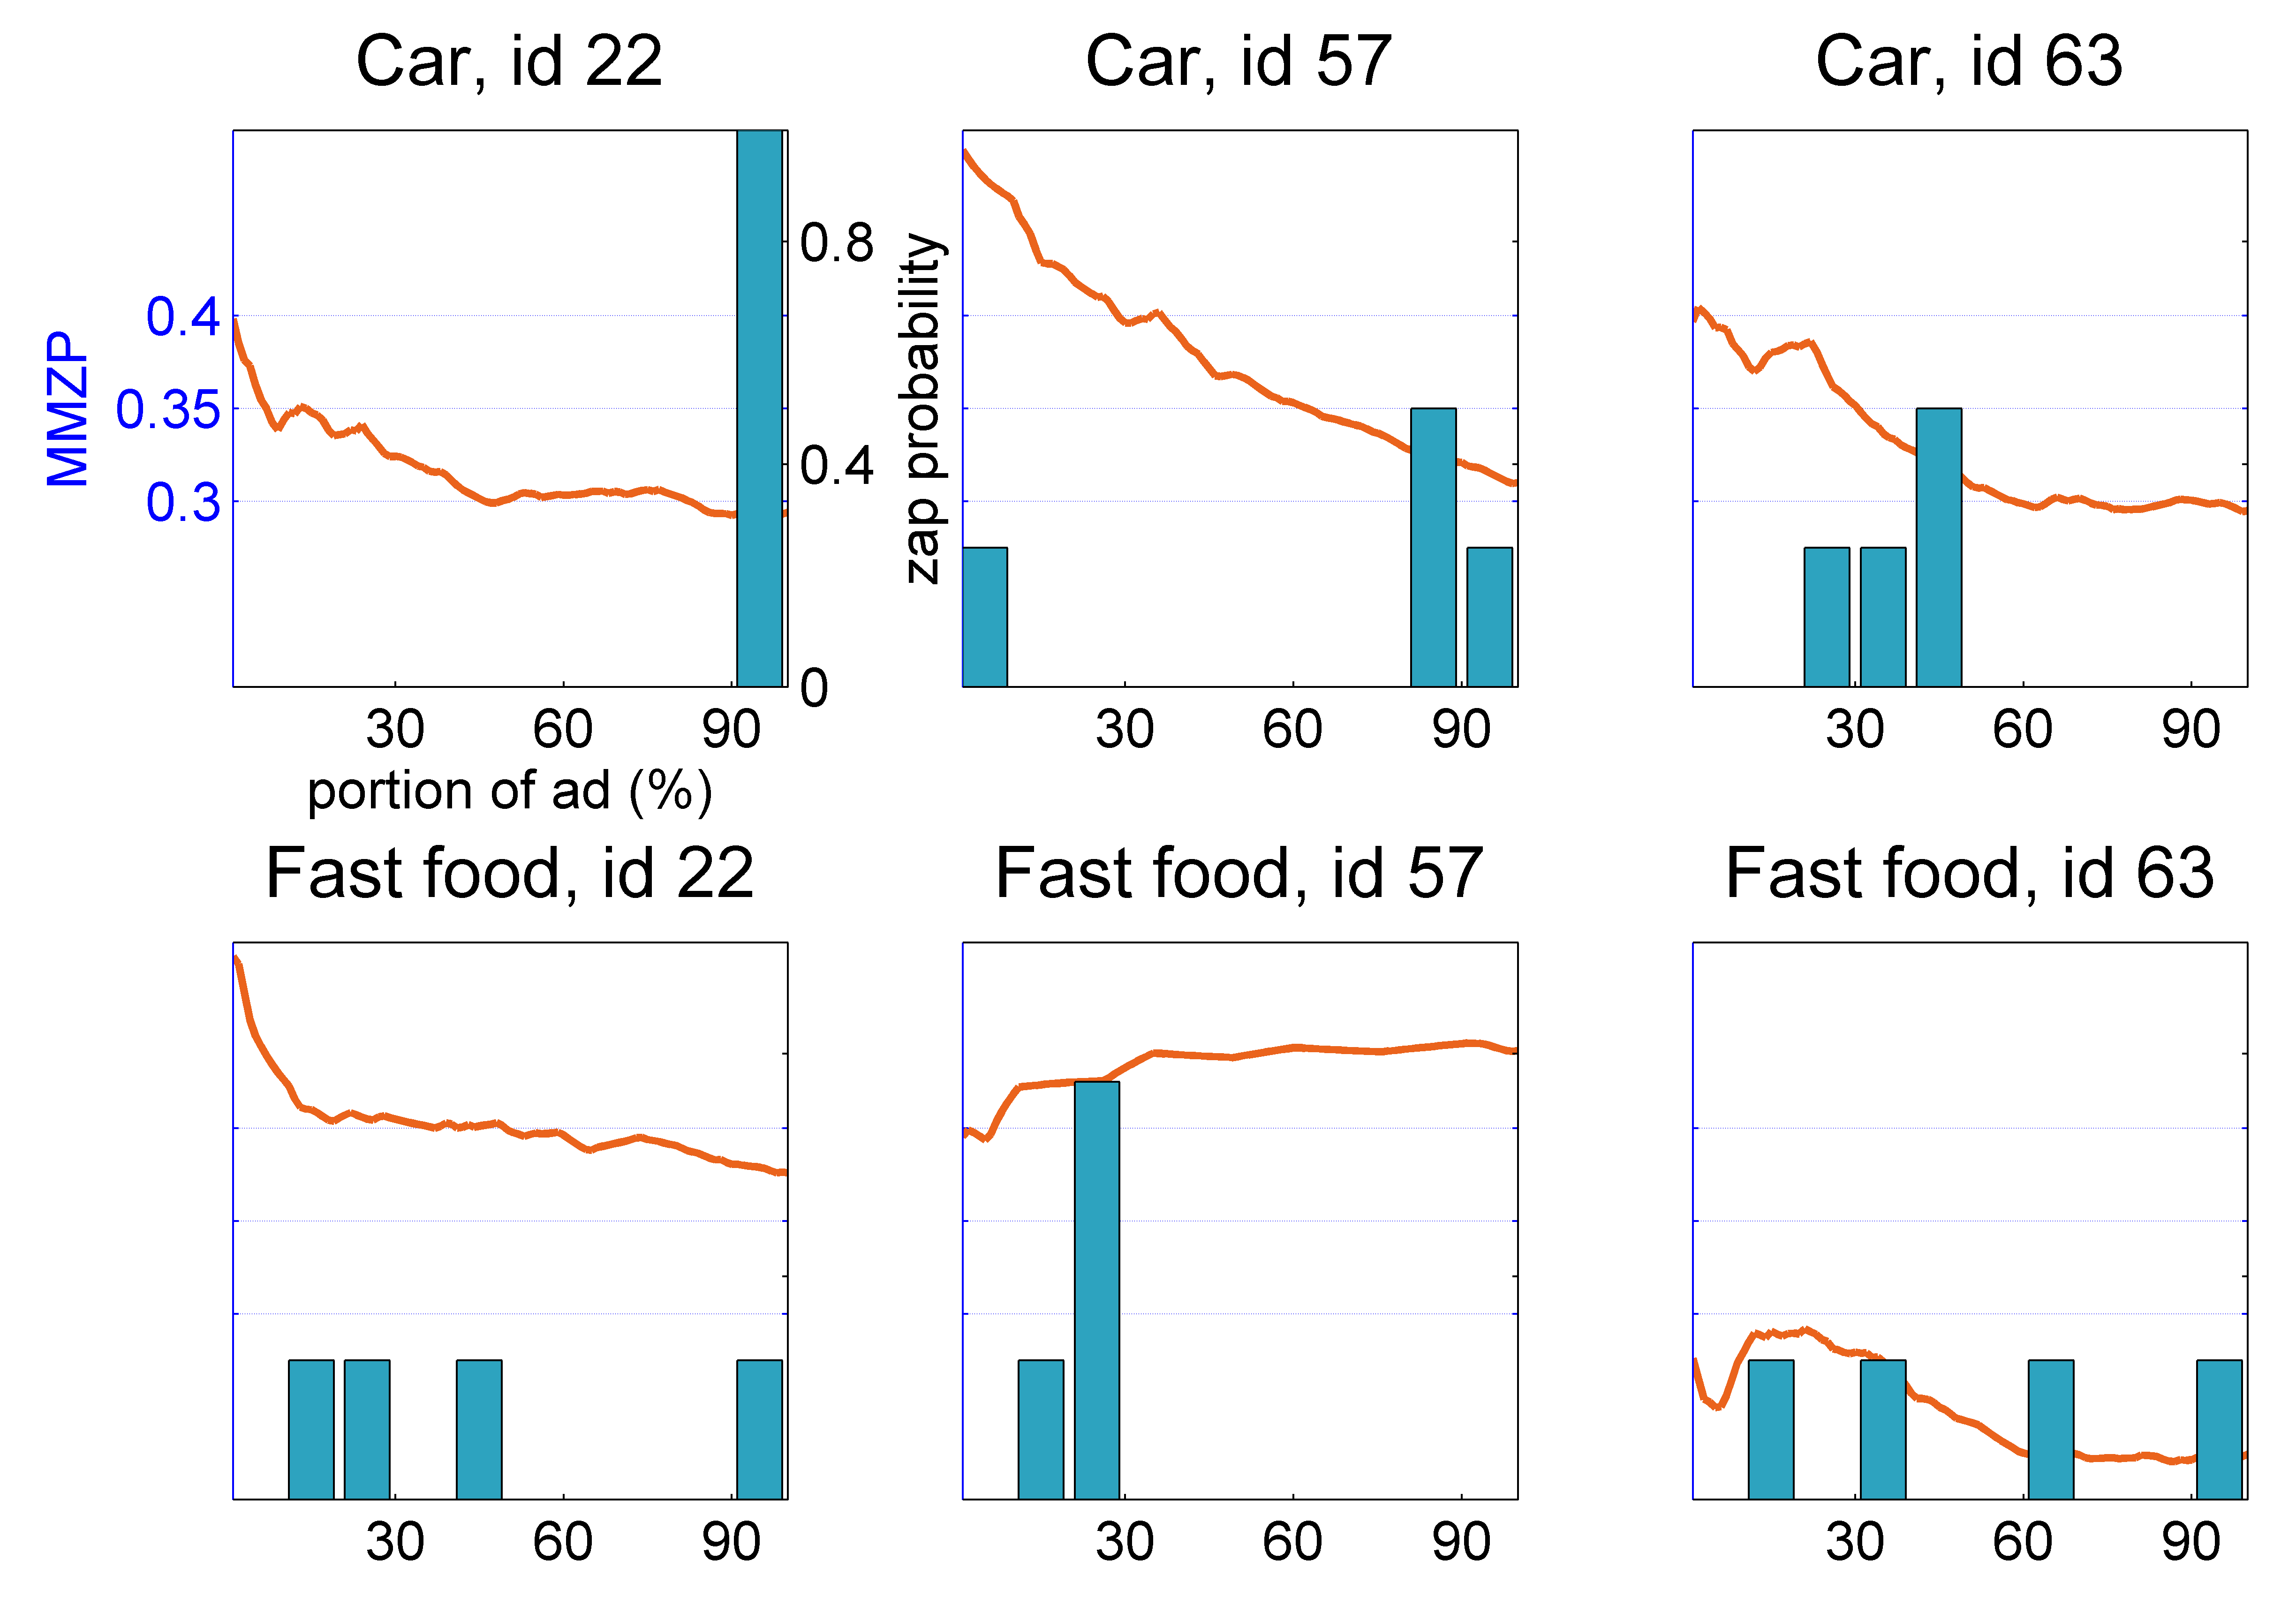
\includegraphics[width=\columnwidth]{fig/adcat_id.png}
	\caption{Examples of personal zapping behavior. It is observed that subject 22 and 57 prefer \textit{Car} ads while subject 63 likes \textit{Fast Food} ads better.}
	\label{fig:adcat_id}
\end{figure}


\noindent \textbf{Personalized User Preference for Ads.} Targeted advertising has proven to be effective in online marketing, as evidenced by the dissemination of online personalized recommendations. We argue that the proposed MMZP can also be used as a user preference metric and therefore, has the potential to help with better personalized advertising. In Fig.~\ref{fig:adcat_id} we show three subjects' MMZP from watching ads in both categories. The decreasing MMZP towards the end of an ad for subject 22 and 57 suggests that they prefer \textit{Car} ads more than \textit{Fast food} ads in which their MMZP remains high across the sequence. On the other hand, based on the changes in MMZP, subject 63 is more interested in \textit{Fast food} than \textit{Car}. These observations are also confirmed by the corresponding ground truth zapping distribution. Thus, using MMZP can provide a better understanding of personal zapping behavior, which is essential for more accurate personalized ad targeting.


\section{Conclusions}

Online user behavior analysis plays an important role in marketing and advertising. In this paper, we have proposed a metric termed moment-to-moment zapping probability (MMZP) for user behavior modeling and understanding based on users' facial expressions. Studies showed that MMZP can be predicted using the smile responses, and knowledge regarding user behavior and preference can be discovered from MMZP. The findings by analyzing the MMZP may facilitate better group-specific or even person-specific advertisement design and targeting. 


\bibliographystyle{ieee}
\bibliography{AdEmo}

\end{document}

% End of ltexpprt.tex